\documentclass[12pt,titlepage]{article}
\usepackage[table]{xcolor}
\usepackage{longtable}
\usepackage[utf8]{inputenc}
%Language of Document Elements like Figure or Table
\usepackage[english]{babel}
\usepackage[bookmarks]{hyperref}
\usepackage{pdfpages}
\usepackage{graphicx}
\usepackage{float}
\usepackage{colortbl,array}
\usepackage[justification=centering]{caption}
\usepackage{enumitem}
\usepackage{chngcntr}
\usepackage{lscape}
\usepackage{fancyhdr}
\usepackage{listings}
\usepackage{hyperref}
\usepackage{nameref}
\usepackage{tabularx}
\usepackage[a4paper,width=160mm,top=25mm,bottom=25mm]{geometry}
\usepackage[ngerman]{translator}
\usepackage{acronym}
\usepackage{listings}
\usepackage{makecell}


\definecolor{warningbackground}{RGB}{252,226,158}

\newcommand{\alertwarningbox}[1]{
	\begin{tabularx}{\linewidth}{
			>{\columncolor{warningbackground}}c
			>{\columncolor{warningbackground}}X}
		\raisebox{\dimexpr2\baselineskip-\height} &
		\raisebox{\tabcolsep}{\strut}#1\raisebox{-\tabcolsep}{\strut}
	\end{tabularx}
}

%Syntax-highlighting]
%\usepackage{minted}
%\usemintedstyle{vs}

%Each Section in a new Page
\let\oldsection\section
\renewcommand\section{\clearpage\oldsection}

%Set space around and between lists
\setlist[enumerate]{noitemsep, topsep=0cm}
\setlist[itemize]{noitemsep, topsep=0cm}

%Figure/Table Numbering style "Section Number.figure counter
\renewcommand{\thefigure}{\arabic{section}.\arabic{figure}}
\renewcommand{\thetable}{\arabic{section}.\arabic{table}}

%Reset figure/table counter after section change
\counterwithin{figure}{section}
\counterwithin{table}{section}

\hypersetup{
	colorlinks,
	linkcolor={black},
	citecolor={black},
	urlcolor={black}
}

\colorlet{punct}{red!60!black}
\definecolor{background}{HTML}{EEEEEE}
\definecolor{delim}{RGB}{20,105,176}
\colorlet{numb}{magenta!60!black}

\newcommand{\todonl}[1]{\newline\textcolor{red}{TODO: #1}\PackageWarning{TODO:}{#1!}}
\newcommand{\todo}[1]{\textcolor{red}{TODO: #1}\PackageWarning{TODO:}{#1!}}

%Set Paragraph indent to null
\setlength{\parindent}{0pt}
% Smaler Table Space
\renewcommand{\arraystretch}{1.5}

% renamig of section to Abschnitt \autoref
\addto\extrasenglish{%
	\def\sectionautorefname{Abschnitt}%
}

% renamig of subsubsection to Abschnitt \autoref
\addto\extrasenglish{%
	\def\subsubsectionautorefname{Abschnitt}%
}

% renamig of subsection to Abschnitt \autoref
\addto\extrasenglish{%
	\def\subsectionautorefname{Abschnitt}%
}
%rename Figure zu Abbildung
\addto\captionsenglish{\renewcommand{\figurename}{Abbildung}}

%rename Tabe zu Tabelle
\addto\captionsenglish{\renewcommand{\tablename}{Tabelle}}

\title{Software-Defined Netzwerk im Campus Bereich}
\author{Sandro Kaspar, Philipp Albrecht, Jessica Kalberer}
\date{28.02.2017}

\pagestyle{fancy}
\lhead{Software-Defined Netzwerk im Campus Bereich}
\begin{document}
\pagenumbering{Roman}


\includepdf{pdfincludes/titlepage}

\newpage
%new Title for tableofcontent
\renewcommand{\contentsname}{Inhaltsverzeichnis}
\tableofcontents
\newpage
\pagenumbering{arabic}

\section{Aufgabenstellung}
Dies ist die initiale Aufgabenstellung, welche zu Beginn der Studienarbeit vorlag. 

\begin{figure}[H]
	\centering
	\includegraphics[height=16cm]{img/aufgabenstellung.jpg}
	\caption{Aufgabenstellung aus AVT \cite{avt-tool}}
	\label{fig:Aufgabenstellung}
\end{figure}

Die Zielsetzungen der initialen Aufgabenstellung wurden nach Absprache mit dem Betreuer anhand der Erkentnisse im Verlauf der Studienarbeit angepasst. Die aktualisierte Aufgabenstellung mit den dazugehörigen Zielsetzungen sind im Abstract ersichtlich (Siehe: \ref{Abstract} Aufgabenstellung).

\section{Abstract}
Der Abstract richtet sich an den Spezialisten auf dem entsprechenden Gebiet und 
beschreibt daher in erster Linie die (neuen, eigenen) Ergebnisse und Resultate der 
Arbeit. Es umfasst nie mehr als eine Seite, typisch sogar nur etwa 200 Worte (etwa 
20 Zeilen). Es sind keine Bilder zu verwenden.

\subsection{Version 2}

Ziel dieser Studienarbeit war die Evaluation der Software Defined Access Lösung von Cisco für die Führungsunterstützungsbasis der Schweizer Armee. Der erste Schwerpunkt lag dabei auf der Installation des Cisco Digital Network Architecture (DNA) Centers und der Konfiguration sowie Integration eines Campus Netzwerkes. Für das DNS-, DHCP- und IP-Adress-Management (IPAM) wird im Campus Netzwerk Infoblox eingesetzt. Für die Benutzerverwaltung sowie Zugriffskontrolle wird die Cisco Identity Services Engine (ISE) verwendet.

Nach dem Einrichten des Campus Netzwerkes lag der zweite Schwerpunkt auf der Definition von Benutzer- und Geräteprofilen, um den einzelnen Mitarbeitern der Schweizer Armee den Netzwerkzugriff zu ermöglichen und die Zugriffsrechte der einzelnen Mitarbeiter oder eines Teams zentral zu regeln. Des Weiteren sollte mit DNA Assurance eine proaktive Überwachung, Fehlerbehebung und Optimierung des Netzwerkes sichergestellt werden. Mit diesen Informationen sollten wöchentliche Reports über den Status des Netzwerks per E-Mail oder Slack Message versendet werden.\\
\\
Die Inbetriebnahme des Campus Netzwerkes gestaltete sich schwieriger als erwartet. Viele der Schritte sind nur teilweise automatisiert und es ist sehr viel manueller Aufwand nötig. Als Beispiel kann hier die LAN Automation aufgeführt werden. Mit Hilfe dieser sollten sich Netzwerkgeräte automatisiert via PnP in Betrieb nehmen und konfigurieren lassen. Dieser Prozess ist allerdings sehr fehleranfällig und funktioniert nur unzuverlässig, sodass die Inbetriebnahme des Underlay Netzwerkes erst nach mehreren Versuchen korrekt ausgeführt werden konnte. 
Des Weiteren funktionieren viele Funktionen des DNA Centers nur mit spezifischen Versionen von ISE und IOS-XE. Dies führte zu weiteren Komplikationen, da dies vom Hersteller so nicht dokumentiert ist. 
Durch diese Komplikationen wurde der ganze Provisionierungsprozess verzögert. 
\\
Abschliessend kann gesagt werden, das für die Installation und Konfiguration des DNA Centers mehrere Tage, wenn nicht Wochen eingerechnet werden müssen. Zudem muss im optimalen Fall ein Green Field vorliegen, da zur Zeit kein bestehendes Netzwerk ohne Unterbrüche migriert werden kann. Bei der Installation sollten die empfohlenen Softwareversionen genauestens eingehalten werden, da sonst die volle Funktionalität des DNA Centers nicht gewährleistet werden kann. Beim Kauf des DNA Centers ist es am einfachsten, gleich auch einen Experten von Cisco aufzubieten, um diese Appliance komplett in der gewünschten Umgebung in Betrieb zu nehmen. 

%\subsection{Ausgangslage}

%\subsection{Ziele der Arbeit}
%Das grundsätzliche Ziel ist eine Evaluation des Cisco Software Defined Networking. Im ersten Schritt beinhaltet das die %Inbetriebnahme und Konfiguration von den folgenden Komponenten:
%\begin{itemize}
%	\item Cisco DNA Center Appliance
%	\item Integration Infoblox (One Platform Solution für DNS, DHCP, IPAM)
%	\item Integration Cisco ISE (Access and Authentification Control)
%	\item Integration Campus Labor Netzwerk
%\end{itemize}
%Im zweiten Schritt sollen UseCases durchgespielt werden, die den folgenden Umfang abdecken:
%\begin{itemize}
%	\item Definierung von Benutzer- und Geräteprofile, um basierend auf Geschäftsanforderungen die Zugriffsrechte und Netzwerksegmentierung zu verwalten und so das Netzwerk sicher zu halten.
%	\item DNA Analytics and Assurance für eine proaktive Überwachung, Fehlerbehebung und Optimierung des Netzwerks.
%	\item IP Address Management Tool im DNA Center.
%	\item Wöchentliche Reports über Campus Netzwerk-Status via E-Mail oder Slack
%\end{itemize}

%\subsection{Ergebnisse}

\section{Management Summary}

\subsection{Ausgangslage}
Diese Arbeit beschäftigt sich mit Software Defined Networking im Campus LAN für die Führungsunterstützungsbasis der Schweizer Armee. Die Lösung soll den Netzwerkzugriff der Mitarbeiter der FUB sicherstellen und die Zugriffsrechte der einzelnen Mitarbeiter oder Teams regeln können. 
Des Weiteren müssen Reportingfunktionion und eine proaktive Überwachung erstellt werden, um allfällige Fehler schnellstmöglich zu erkennen, das Netzwerk stets zu optimieren und dessen Funktion jederzeit sicherzustellen.
Zusätzlich wird ein bestehends IP Management Tool in die Lösung integriert.

Da die Anforderungen an Campus Netzwerke aus verschiensten Gründen, wie z.Bsp. modernen Arbeitsmodellen, neuen Sicherheitsanforderungen usw. ständig steigen, ist es äusserst schwierig und aufwändig, diese Anforderungen mit traditionellen Methoden zu erfüllen. 

Um dies zu erreichen, wird in dieser Arbeit daher ein Software Defined Network erstellt, dass diesen neuen Anforderungen gerecht werden soll. Vorteile zeigen sich insbesondere dadurch, dass eine derartige Lösung flexibler ist, also einfacher und schneller an neue Gegebenheiten angepasst werden kann und durch Schnittstellen einfach an bestehende Systeme anzubinden ist. Durch das zentrale Management und Monitoring der Komponenten sinkt zudem das Risiko für Fehler massiv und viele Aufgaben lassen sich einfach und schnell automatisieren.
Schlussendlich kann durch diese Vorteile sehr viel Aufwand und damit Kosten eingespart werden.

Ziel ist es, die Vorteile dieser Lösung gegenüber einer traditionellen Netzwerkinfrastruktur aufzuzeigen, allfällige Risiken und mögliche Probleme früh zu erkennen und Lösungen für diese zu finden. 
\subsection{Vorgehen und Technologien}
Die Lösung wird mit dem Produkt Software Defined Access von Cisco erstellt. Diese besteht aus mehreren Komponenten dies ist zum einem das DNA Center, welches die grundsätzliche Funktion des Netzwerks sicherstellt, sowie ISE (Identity Service Engine), welches die Benutzeridentitäten und Profile verwaltet.
Zusätzlich muss das bestehende IP Management in die Lösung integriert werden und Reporting Funktionen mittels Slack und E-Mail implementiert werden. Diese Zusatzfunktionalitäten werden in Python implementiert und nutzen die in Ciscos SDA enthaltenen APIs.
\subsection{Ergebnisse}
Am Ende dieser Arbeit wird ein funktionierender Prototyp eines Software Defined Networks im Access Bereich zur Verfügung stehen, der alle Requirements des Industriepartners abdeckt. Der Prototyp besteht aus den Cisco Komponenten, sowie Eigenentwicklungen, die zusätzliche Features implementieren. 
Zudem steht eine Dokumentation des Systems zur Verfügung, die den Installationsprozess und die Handhabung des Systems erklärt. Des Weiteren zeigt die Dokumentation Vorteile, aber auch Risiken und mögliche Probleme im Vergleich zu einer traditionellen Netzwerklösung auf.
\subsection{Ausblick}
Die Resultate aus dieser Arbeit können dazu dienen, SDA in einer produktiven Umgebung in Betrieb zu nehmen. Zudem kann er Prototyp um zusätzliche Funktionen erweitert werden, an zusätzliche bestehende oder neue Systeme angebunden werden oder mit alternativen Lösungen verglichen werden.

\section{Ausgangslage (Kontext)}

\begin{itemize}	
	\item Beschreibung des Typs der Arbeit (Bsp. Fokus Lösungserstellung oder Machbarkeitsanalyse)
	\item Fachliche Domäne, Zielgruppe, heutige Praktiken bzw. Lösungen (Methoden, Tools, etc.)
\end{itemize}


\section{Problembeschreibung}
Wer den heutigen Anforderungen der Campus Netzwerke in Bezug auf Sicherheit, Wartbarkeit und Skalierbarkeit gerecht werden möchte, steht mit der isolierten Konfiguration einzelner Komponenten schnell vor verschiedenen Problemen. In erster Linie ist es extrem aufwändig, alle Konfigurationen manuell zu erstellen. Selbst das Hinzufügen von einfachen Richtlinien oder neuen Firmenabteilungen kann zu gewaltigem Aufwand führen. Des Weiteren kann die Übersicht schnell verloren werden und eine umfangreiche Dokumentation zu erstellen ist unumgänglich. Häufig kommen selbstgeschriebene Scripts, zum Beispiel mithilfe von NAPALM \cite{napalm} zur automatisierten Konfiguration zum Einsatz. Für das Monitoring des Netzwerkes sind zusätzlich Tools wie icinga2 \cite{icinga2} oder ähnliches nötig. 

~\\
Typische Herausforderungen bei den klassischen Campus Netzwerken:
\begin{itemize}
	\item Zu wenig VLANs
	\item Mobilität von Endgeräten
	\item Mobilität von Benutzern
	\item Durchsetzen von Sicherheitsregeln mithilfe von Firewalls
	\item Direkte Abhängigkeit von Berechtigungen und IP Subnetzen
	\item Mehrere unabhängige Tools mit Informationsredundanz
	\item Komplexe Fehlersuche über verschiedene Komponenten/Geräte hinweg
\end{itemize}

~\\
Genau hier setzt das Cisco DNA Center an. Es fasst alle diese Tools unter einem Dach zusammen und bietet eine übergreifende Plattform. 


\section{Lösungskonzept}

\begin{itemize}	
	\item Dokumentation Architektur und Design (i.d.R. plattformneutral bzw. technologieübergreifend, z.B. in Form von UML-Diagrammen und Erläuterungen dazu) 
	\item Architekturentscheidungen mit Begründungen
	\item Diskussion, wie Qualitätsattribute adressiert werden (welche Qualität kann erreicht werden?)
\end{itemize}

\subsection{Technologien}
\subsubsection{Software-Defined Network (SDN)}
SDN ist ein neues Konzept, um Netzwerke zu designen, implementieren und betreiben. Zu den Grundprinzipien des SDN gehören die Entkopplung von Control Plane und Data Plane. Dabei wird die Kontrolle von der Hardware entkoppelt und an eine Software-Anwendung (den Controller) übergeben. Darüber hinaus werden die Netzwerkinfrastruktur und Netzwerkanwendungen getrennt. SDN gibt den Netzadministratoren eine programmierbare, zentrale Steuerung des Netzverkehrs, ohne manuell Zugriff auf die einzelnen physischen Netzkomponenten nehmen zu müssen. Zur Implementierung eines SDN gibt es drei Ansätze:
\begin{itemize}
	\item Switch-basiertes Modell
	\item Overlay-Modell
	\item Hybrid-Ansatz
\end{itemize}

\subsubsection{Cisco Digital Network Architecture Center (Cisco DNA-Center)}

\subsubsection{Locator ID Separation Protocol (LISP)}
LISP ist das Produkt einer Arbeitsgruppe in der Internet Engineering Taskforce (IETF), um was wachsende Problem des doppelten Verwendungszwecks der IP-Adressen zu bereinigen. Zur Zeit wird die IP-Adresse benutzt um die Identität eines Hosts festzulegen und auch den Ort zu bestimmen, an dem er sich im Internet befindet. Dies hat zur Folge das sich bei einem Aufenthalsortwechsel auch die IP-Adresse des Hosts ändert, was bedeutet das die Identität verloren geht und die alten IP-Verbindungen verfallen. \\

Dies soll nun durch LISP geändert werden, in dem es die Identität eines Gerätes, auch Endpoint Identifier (EID) genannt, von seinem Aufenthaltsort, auch Routing Locator (RLOC) genannt, in zwei separate Adressräume unterteilt. Das bedeutet, dass die Router in einer LISP-Architektur nur Routing-Informationen von RLOCs speichern müssen. Um Pfadinformationen eines Hosts abzurufen, kann der Router diese beim LISP-Mapping-Server abfragen, was analog wie das DNS-Mapping funktioniert. \\

LISP verwendet für SDA/Fabric eine VXLAN-Kapselung.

\begin{table}[H]
	\rowcolors{2}{gray!25}{white}
	\centering
	\begin{tabularx}{\textwidth}{p{6.6cm} | X}
		\rowcolor{gray!50}
		\textbf{LISP Device} & \textbf{Function} \\
		\hline	
		ALT (Alternative Logical Topology) & Collects EID data from Map Servers (MS) and advertise aggregate EID prefix. In a deployment of multiple Map Servers, it keeps all synchronized. \\
		
		ETR (Egress Tunnel Router) and PETR (Proxy ETR) & Connects a LISP capable core network. Registers EID prefices with Map Server (MS). Decapsulates LISP packets, received from LISP core. Responds to Map-request messages with a Map-Reply by giving appropriate EID prefix. Typically, this is a CPE (customer premise equipment) router. PETR works on behalf on non-LISP domain and provides LISP-non-LISP connectivity. \\ 
		
		ITR (Ingress Tunnel Router) and PITR (Proxy Ingress Tunnel Router) & Responsible for forwarding local traffic to external destinations. Resolves RLOC for a given destination by sending Map-request to Map Resolver. Encapsulates (vxlan) traffic with LISP header. Typically, this is a Access Layer Switch. PITR works on behalf on non-LISP domain and provides LISP-non-LISP connectivity. \\
		
		XTR (X Tunnel Router) & When both ITR and ETR functions are handled by one router, it is called XTR. This is typical in practice. \\
		
		MR (Map Resolver) & Responds to Map-requests from ITR. Map-requests will be replied with a Negative Map-Reply or forwarded to appropriate ETR or ALT. \\
		
		MS (Map Server) & Registers EID space upon receiving Map-register messages from ETR. Updates ALT and MR with EID and RLOC data. \\
		
		MSMR (Map Server Map Reloader) & When a device acts as both Map Server and Map Resolver, it is called MSMR. This is typical in practice. \\
		
		EID (Endpoint ID) & Endpoint Identifier. IP addresses hidden from core network routing table. RLOC acts next-hop to reach EID space. \\
		
		RLOC (Routing Locator) & Routing Locator. Exists in global routing tables. Authoritative to reach EID space. \\
		               
	\end{tabularx}
	\caption{LISP Elements}
	\label{tab:my-label}
\end{table}

\subsubsection{Virtual Extensible LAN (VXLAN)}
VXLAN ist ein Encapsulation-Protokoll, um ein Overlay-Netzwerk auf einer existierenden Layer 3 Infrasturktur laufen zu lassen. VXLAN wurde ursprünglich von Cisco Systems, VMware und Arista Network entwickelt und ist einer der IETF festgelegten Standards (RFC 7348). \\
\\
Technisch gesehen erzeugt ein VXLAN logische Layer 2 Netzwerke, die dann in standardmässige Layer 3 Pakete eingepackt werden. VXLAN dient dazu um in sehr grossen Netzwerkumgebung die Probleme zu lösen, die durch beschränkte Anzahl von VLANS betroffen sind. Mit VXLAN sind insgesamt 16’777’215 (24 Bit) Layer-2-Umgebungen möglich, die ihrerseits wieder jeweils 4096 VLANs beinhalten können.
\section{Technologien}

\subsection{Software Defined Access (SDA)}
Cisco bietet mit SDA eine automatisierte End-to-End-Segmentierung um den Benutzer-, Geräte- und Anwendungsverkehr zu trennen, ohne das Netzwerk neu zu gestalten. Durch diesen automatisierten Benutzerzugriff ermöglicht SDA Einrichtungen innert kürzester Zeit. Durch diese enorme Vereinfachung wird eine zusätzliche Sicherheit und Skalierung des Betriebs gewonnen. Ebenso wird die Transparenz deutlich erhöht und die schnelle Bereitstellung neuer Dienste gewährleistet. Durch die Automatisierung von täglichen Aufgaben wie Konfiguration, Bereitstellung und Troubleshooting reduziert SDA die Zeit für Netzwerkanpassungen, verbessert die Problemlösungszeit und reduziert die Auswirkungen von Sicherheitsverletzungen.\\
\\
So können Organisationen sicherstellen, dass für jeden Benutzer oder jedes Gerät mit jeder Anwendung die richtigen Richtlinien festgelegt werden über das Netzwerk. Dies wird mit einer einzigen Netzwerkstruktur über LAN und WLAN erreicht, wodurch ein konsistente Benutzererfahrung überall ohne Kompromisse bei der Sicherheit. \\
\\
SDA wird aus mehreren Komponenten zusammengesetzt. Dazu gehört das DNA-Center, welches die grundsätzliche Funktion des Netzwerks sicherstellt, sowie Identity Service Engine (ISE), welches die Benutzeridentitäten und Profile verwaltet.

\subsubsection{Campus Fabric}
Um eine konsistente Benutzererfahrung zu erreichen, braucht man eine Switching-Infrastruktur mit der sich der Zugang zu bestimmten IP-Subnetzen ortsunabhängig realisieren lässt.

Cisco hat nun ein neues Overlay für diesen Zweck erfunden, die "Campus Fabric". Das Overlay ist hierbei eine Kombination aus LISP und VXLAN.

\begin{figure}[H]
	\centering
	\includegraphics[height=6cm]{img/campusfabric.jpg}
	\caption{Campus Fabric}
	\label{fig:Campus Fabric}
\end{figure}

Die Fabric bildet ein Overlay Netz. Das Overlay Netz bildet eine virtuelle Topologie um Geräte miteinander zu verbinden, welches auf einer beliebigen physischen Underlay Topologie aufgebaut ist. Das Overlay Netzwerk verwendet oft alternative Weiterleitungsattribute, um zusätzliche Dienste bereitzustellen, die nicht vom Underlay Netzwerk bereitgestellt werden.

In der nachfolgenden Abbildung ist der Aufbau eines Campus Fabric etwas detaillierter aufgezeigt.

\begin{figure}[H]
	\centering
	\includegraphics[height=8cm]{img/fabric-roles&terminology.jpg}
	\caption{Fabric Rollen und Terminologie}
	\label{fig:Fabric Rollen und Terminologie}
\end{figure}

Dieses Campus Fabric besteht aus folgenden Elementen:
\begin{itemize}	
	\item User/Group Repository: Ein externes ID-Speichergerät (z. B. ISE oder AD) kann verwendet werden, um eine dynamische Zuordnung von Benutzer/Gerät zu Gruppen bereitzustellen
	\item Control-Plane-Nodes: Ein Map System, das die Beziehung eines Endpoints zu einem Gateway (Edge oder Border) verwaltet
	\item Border-Nodes: Das L3-Gateway-Gerät (Core), das externe L3-Netzwerke mit dem Fabric verbindet
	\item Edge-Nodes: Das L3-Gateway-Gerät (Access oder Distribution), das Endpoints mit Fabric verbindet
	\item Intermediate Nodes: Normale L3 (IP) Forwarder im Underlay Netzwerk
\end{itemize}

\subsection{Cisco Digital Network Architecture Center (Cisco DNA-Center)}
DNA Center ist das zentrale Überwachungs-Dashboard für Netzwerke, mit dem alle Cisco DNA-Produkte und -Lösungen verwaltet werden können.
DNA Center gibt die Möglichkeit unter einem Grafischen Nutzer Interface direkt mit APIC(Application Policy Infrastructure Controller)-EM 2.x Applikationen mit der Identity Services Engine (ISE) und mit Network Data Plattform (NDP) unserer Assurance und Analytics Plattform zu sprechen. Alle Parameter die angezeigt oder konfiguriert werden müssen kann man unter DNA Center ausführen und muss nicht zwischen den einzelnen Modulen und Oberflächen hin und her springen.
\begin{figure}[H]
	\centering
	\includegraphics[height=8cm]{img/DNAC-1.jpg}
	\caption{DNA Solution}
	\label{fig:Aufbau einer DNA Solution}
\end{figure}
APIC-EM 2.x automatisiert dann die notwendigen Konfigurationen und spricht mit dem Netzwerk. Auch die Integration von IP Address Management Lösungen wie zB Infoblox werden nur über die DNA Center Oberfläche konfiguriert. \\
\\
SD-Access ist die Grundlage von Cisco DNA. Es ermöglicht Netzwerkzugriff in Minuten für jeden Benutzer oder jedes Gerät für jede Anwendung, ohne Kompromisse. Bei SD-Access folgen die festgelegten Richtlinien automatisch dem Benutzer über alle Netzwerkdomänen hinweg.

\subsection{Identity Service Engine (ISE)}
Mit der Cisco ISE können Benutzer und Geräte, die mit dem Unternehmensnetzwerk verbunden sind, angezeigt und gesteuert werden. Das alles von einer zentralen Stelle aus. ISE ermöglicht es einem Netzwerkadministrator, Zugriffsrichtlinien für kabelgebundene und drahtlose Endpunkte basierend auf Informationen zentral zu steuern, die über RADIUS-Nachrichten gesammelt werden, die zwischen dem Gerät und dem ISE-Knoten übertragen werden. Dies wird auch als Profiling bezeichnet. Die Profiling-Datenbank wird regelmäßig aktualisiert, um mit den neuesten und besten Geräten Schritt zu halten, so dass keine Lücken in der Gerätesichtbarkeit bestehen. \\
\\
Im Wesentlichen hängt ISE eine Identität an ein Gerät an, basierend auf Benutzer-, Funktions- oder anderen Attributen, um Richtliniendurchsetzung und Sicherheitskonformität bereitzustellen, bevor das Gerät autorisiert wird, auf das Netzwerk zuzugreifen. Basierend auf den Ergebnissen einer Vielzahl von Variablen kann ein Endpunkt mit bestimmten Zugriffsregeln auf das Netzwerk zugelassen werden, die auf die Schnittstelle angewendet werden, mit der er verbunden ist. Andernfalls kann er vollständig verweigert oder basierend auf den spezifischen Unternehmensrichtlinien gewährt werden. \\
\\
DNA Center bietet einen Mechanismus zum Erstellen einer vertrauenswürdigen Kommunikationsverbindung mit Cisco Identity Services Engine (ISE) und ermöglicht den beiden Anwendungen, Daten auf sichere Weise miteinander zu teilen. Sobald die ISE beim DNA Center registriert ist, wird jedes Gerät, das ISE entdeckt, zusammen mit der entsprechenden Konfiguration und anderen Daten an das DNA Center weitergeleitet. Benutzer können beide Anwendungen verwenden, um Geräte zu erkennen und dann sowohl DNA Center- als auch ISE-Funktionen auf sie anzuwenden, da diese Geräte in beiden Anwendungen verfügbar sind. DNA Center- und ISE-Geräte werden alle durch ihre Gerätenamen eindeutig identifiziert. \\
\\
In ähnlicher Weise werden DNA-Center-Geräte, sobald sie bereitgestellt werden und zu einer bestimmten Site in der DNA Center-Standorthierarchie gehören, an ISE übergeben. Alle Aktualisierungen an einem DNA Center-Gerät (z. B. Änderungen an der IP-Adresse, SNMP- oder CLI-Anmeldeinformationen, gemeinsamer ISE-Schlüssel usw.) werden automatisch an die entsprechende Geräteinstanz auf der ISE weitergeleitet. Wenn ein DNA Center-Gerät gelöscht wird, wird es ebenfalls aus der ISE entfernt.

\subsection{Locator ID Separation Protocol (LISP)}
LISP ist das Produkt einer Arbeitsgruppe in der Internet Engineering Taskforce (IETF), um was wachsende Problem des doppelten Verwendungszwecks der IP-Adressen zu bereinigen. Zur Zeit wird die IP-Adresse benutzt um die Identität eines Hosts festzulegen und auch den Ort zu bestimmen, an dem er sich im Internet befindet. Dies hat zur Folge das sich bei einem Aufenthalsortwechsel auch die IP-Adresse des Hosts ändert, was bedeutet das die Identität verloren geht und die alten IP-Verbindungen verfallen. \\

Dies soll nun durch LISP geändert werden, in dem es die Identität eines Gerätes, auch Endpoint Identifier (EID) genannt, von seinem Aufenthaltsort, auch Routing Locator (RLOC) genannt, in zwei separate Adressräume unterteilt. Das bedeutet, dass die Router in einer LISP-Architektur nur Routing-Informationen von RLOCs speichern müssen. Um Pfadinformationen eines Hosts abzurufen, kann der Router diese beim LISP-Mapping-Server abfragen, was analog wie das DNS-Mapping funktioniert. \\

LISP verwendet für SDA/Fabric eine VXLAN-Kapselung.

\begin{table}[H]
	\rowcolors{2}{gray!25}{white}
	\centering
	\begin{tabularx}{\textwidth}{p{6.6cm} | X}
		\rowcolor{gray!50}
		\textbf{LISP Device} & \textbf{Function} \\
		\hline	
		ALT (Alternative Logical Topology) & Collects EID data from Map Servers (MS) and advertise aggregate EID prefix. In a deployment of multiple Map Servers, it keeps all synchronized. \\
		
		ETR (Egress Tunnel Router) and PETR (Proxy ETR) & Connects a LISP capable core network. Registers EID prefices with Map Server (MS). Decapsulates LISP packets, received from LISP core. Responds to Map-request messages with a Map-Reply by giving appropriate EID prefix. Typically, this is a CPE (customer premise equipment) router. PETR works on behalf on non-LISP domain and provides LISP-non-LISP connectivity. \\ 
		
		ITR (Ingress Tunnel Router) and PITR (Proxy Ingress Tunnel Router) & Responsible for forwarding local traffic to external destinations. Resolves RLOC for a given destination by sending Map-request to Map Resolver. Encapsulates (vxlan) traffic with LISP header. Typically, this is a Access Layer Switch. PITR works on behalf on non-LISP domain and provides LISP-non-LISP connectivity. \\
		
		XTR (X Tunnel Router) & When both ITR and ETR functions are handled by one router, it is called XTR. This is typical in practice. \\
		
		MR (Map Resolver) & Responds to Map-requests from ITR. Map-requests will be replied with a Negative Map-Reply or forwarded to appropriate ETR or ALT. \\
		
		MS (Map Server) & Registers EID space upon receiving Map-register messages from ETR. Updates ALT and MR with EID and RLOC data. \\
		
		MSMR (Map Server Map Reloader) & When a device acts as both Map Server and Map Resolver, it is called MSMR. This is typical in practice. \\
		
		EID (Endpoint ID) & Endpoint Identifier. IP addresses hidden from core network routing table. RLOC acts next-hop to reach EID space. \\
		
		RLOC (Routing Locator) & Routing Locator. Exists in global routing tables. Authoritative to reach EID space. \\
		
	\end{tabularx}
	\caption{LISP Elements}
	\label{tab:my-label}
\end{table}

\subsection{Virtual Extensible LAN (VXLAN)}
VXLAN ist ein Encapsulation-Protokoll, um ein Overlay-Netzwerk auf einer existierenden Layer 3 Infrasturktur laufen zu lassen. VXLAN wurde ursprünglich von Cisco Systems, VMware und Arista Network entwickelt und ist einer der IETF festgelegten Standards (RFC 7348). \\
\\
Technisch gesehen erzeugt ein VXLAN logische Layer 2 Netzwerke, die dann in standardmässige Layer 3 Pakete eingepackt werden. VXLAN dient dazu um in sehr grossen Netzwerkumgebung die Probleme zu lösen, die durch beschränkte Anzahl von VLANS betroffen sind. Mit VXLAN sind insgesamt 16’777’215 (24 Bit) Layer-2-Umgebungen möglich, die ihrerseits wieder jeweils 4096 VLANs beinhalten können.

\subsection{Slack}
Slack ist ein webbasierter Instant-Messaging-Dienst des US-amerikanischen Unternehmens Slack Technologies zur Kommunikation innerhalb von Arbeitsgruppen. Slack erlaubt, Nachrichten auszutauschen, mit Einzelpersonen oder in einer Gruppe zu chatten sowie gemeinsam Dokumente zu bearbeiten. Andere Online-Dienste wie Dropbox, Google Drive oder GitHub lassen sich in Slack integrieren.

\section{Use Cases}

\subsection{Use Cases Brief}
\subsubsection{UC01: }


\subsubsection{UC02: }

\subsection{Use Cases Fully dressed}
\subsubsection{UC01: }
\begin{table}[H]
	\rowcolors{2}{gray!25}{white}
	\centering
	\begin{tabularx}{\textwidth}{l | X}
		Primary Actor      & x        \\
		\hline
		Beschreibung       & x \\ 
		\hline
		Stakeholders       & x: 
		\newline
		\begin{itemize}	
			\item x
		\end{itemize}              \\
		\hline
		Preconditions      & 
		\begin{itemize}	
			\item x
			\item x
		\end{itemize}  \\
		\hline
		Postconditions     & 
		\begin{itemize}	
			\item x
		\end{itemize}  \\
		\hline
		Main Success Story & 
		1.  \newline
		2.  \newline
		3.  \newline
		\\
		\hline
		Alternative Flows  & 
		2a. x. \newline
		\noindent\hspace*{6mm} 1. x \newline
		\noindent\hspace*{6mm} 2. x 
		\newline
		\noindent\hspace*{6mm} \textit{Wiederhole Schritt 1-2 bis die Angaben valide sind.} \newline
		\\
	\end{tabularx}
	\caption{Fully Dressed UC01}
	\label{tab:UC01}
\end{table}

\section{Umsetzung}

\begin{itemize}
	\item Ausgewählte Implementierungsdetails (Bsp. Algorithmen, Datenstrukturen, Libraries, Architectural Hot Spots)Dokumentation Architektur und Design (i.d.R. plattformneutral bzw. technologieübergreifend, z.B. in Form von UML-Diagrammen und Erläuterungen dazu)
	\item Dokumentation, welche Experimente/Tests durchgeführt wurden und welche Lösungsoptionen aufgrund der Ergebnisse dieser Experimente/Tests verworfen wurden.
\end{itemize}

\subsection{Labor Netzwerk Architektur} \label{subsec:Labor-Netzwerk-Architektur}
Mit der zur Verfügung gestellten Hardware ist die folgende Netzwerk Architektur entstanden.

Folgende zentrale Überlegungen sind eingeflossen:

\begin{itemize}
	\item Campus Netzwerk mit mehreren Gebäuden, um das Wandern von Geräten zu simulieren.
	\item Mischung der zur Verfügung stehenden Switches (Catalyst 9300 \& 3850) in der Fabric Edge Nodes, um Verhalten zu vergleichen.
	\item Management Netzwerk ist inbound. Kabelführung zu jedem Switch ist meistens von den Gegebenheiten in typsichen Gebäuden nicht möglich.
\end{itemize}


\begin{figure}[H]
	\centering
	\includegraphics[width=1\linewidth]{img/LabNetworkArchitecture.png}\\[1px]
	\caption{SDN Netzwerk Architektur}
	\label{fig:LabNetworkArchitecture}
\end{figure}

\subsection{Netzwerkarchitekturen Vergleich}
Hauptunterschiede zwischen der klassischen Netzwerkarchitektur und der "Modernen" Software-Defined Access Architektur. 

\begin{itemize}
	\item Bis zur Fabric Edge Nodes (Vergleichbar mit dem Access Layer) unterliegt ein Layer 3 Netzwerk. 
	\item Kein Einsatz von STP oder VSS auf Distribution Layer notwendig, da das Underlay Netzwerk rein Layer 3 ist und Routing Protokolle (OSPF) zum Einsatz kommen.
	\item Der Distribution Layer nimmt neu als Fabric Intermediate Nodes nur noch die Funktion als Layer 3 Brücke bzw. VXLAN transporteuer ein, anstatt die Grenze zwischen Layer 3 und Layer 2 zu sein. Die Fabric Intermediate Nodes sind optional. 
	\item Während beim klassischen Design die logische Netzwerkarchitektur direkt Abhängig ist von der physikalischen Architektur, wird bei SDN die phykalische Netzwerkarchitektur von der logischen Architektur getrennt. Man spricht dann von der Physical Fabric Topology bzw. Underlay und den entsprechenden Layer 2 bzw. Layer 3 Overlay Network. 
\end{itemize}

\begin{figure}[H]
	\centering
	\includegraphics[width=1\linewidth]{img/LabNetworkArchitecture_Vergleich.png}\\[1px]
	\caption{Netzwerk Architektur Vergleich}
	\label{fig:LabNetworkArchitectureVergleich}
\end{figure}

\subsection{Maximale Skalierungen}
Nachfolgend werden die aktuell maximalen Skalierungen des DNA Centers, sowie der Border und Edge Nodes aufgelistet.
\begin{figure}[H]
	\centering
	\includegraphics[width=1\linewidth]{img/MaximumScale-HACluster.png}\\[1px]
	\caption{DNA Center Maximum Scale Constraints HA Cluster}
	\label{fig:Maximum Scale HACluster}
\end{figure}

\begin{figure}[H]
	\centering
	\includegraphics[width=1\linewidth]{img/MaximumScale-Fabric.png}\\[1px]
	\caption{DNA Center Maximum Scale Constraints Fabric}
	\label{fig:Maximum Scale Fabric}
\end{figure}

\begin{figure}[H]
	\centering
	\includegraphics[width=1\linewidth]{img/MaximumScale-EdgeNode.png}\\[1px]
	\caption{SDA Edge Node Scale Constraints}
	\label{fig:SDA Edge Node Scale Constraints}
\end{figure}

\begin{figure}[H]
	\centering
	\includegraphics[width=1\linewidth]{img/MaximumScale-BorderNode.png}\\[1px]
	\caption{SDA Border Node Scale Constraints}
	\label{fig:SDA Border Node Scale Constraints}
\end{figure}

\pagebreak
\subsection{Verkabelungsplan}
\begin{figure}[H]
	\centering
	\includegraphics[angle=90,width=0.9\linewidth]{img/LabNetworkArchitecture-Interfaces.png}\\[1px]
	\caption{Lab Architecture with physical Interfaces}
	\label{fig:Lab Architecture with physical Interfaces}
\end{figure}



\section{Vorgehen}

\begin{figure}[H]
	\centering
	\includegraphics[height=9cm]{img/vorgehen.png}
	\caption{Übersicht Vorgehen}
	\label{fig:vorgehen}
\end{figure} 

\subsection{DNA Center Initiales Setup}

\subsubsection{Installation}
\label{DNACenterSetup_Installation}
Die Installation des DNA Centers erfolgt direkt an der Konsole oder über die Cisco IMC. Dabei wird die maglev-config-wizard ausgeführt. Dieser Befehl kann im nachhinein jederzeit zur Anpassung der Konfiguration ausgeführt werden. 

Wie in \cite{cisco-dna-installation-guide} Kapitel 2 beschrieben werden folgende Angaben benötigt:
\begin{itemize}
	\item Host IP Adresse
	\item Netmask
	\item Default Gateway IP adress
	\item DNS Servers
	\item Static Routes
	\item HTTPS Proxy
	\item Maglev Mster Node IP
	\item Username, Password und Linux Password
	\item Administration Passphrase (for Web Access)
	\item NTP Servers
	\item Service Subnet
\end{itemize}

Im ersten Schritt \ref{fig:dna-center-install-step-1} wird gewählt, ob ein neues Cluster erstellt werden soll oder einem Beigetreten werden soll. Bei der Testumgebung dieser Arbeit war nur eine Appliance verfügbar, weshalb ausschliesslich "Start a DNA-C Cluster" ausgewählt wurde. 

\begin{figure}[H]
	\centering
	\includegraphics[height=9cm]{img/sc_001.png}
	\caption{DNA Center Configuration Wizard Start}
	\label{fig:dna-center-install-step-1}
\end{figure} 

\begin{figure}[H]
	\centering
	\includegraphics[height=9cm]{img/sc_002.png}
	\caption{DNA Center Configuration Wizard - Entering Management IP}
	\label{fig:dna-center-install-step-4}
\end{figure} 

\begin{figure}[H]
	\centering
	\includegraphics[height=9cm]{img/sc_003.png}
	\caption{DNA Center Configuration Wizard - Entering Authentification Data}
	\label{fig:dna-center-install-step-13}
\end{figure}

\begin{figure}[H]
	\centering
	\includegraphics[height=9cm]{img/sc_004.png}
	\caption{DNA Center Configuration Wizard - DNA Center uses docker}
	\label{fig:dna-center-install-step-install}
\end{figure}


\subsubsection{Setup Accounts}
Nach dem der Wizard die Installation vollständig ausgeführt hat, ist das DNA Center Web-GUI verfügbar.
\begin{figure}[H]
	\centering
	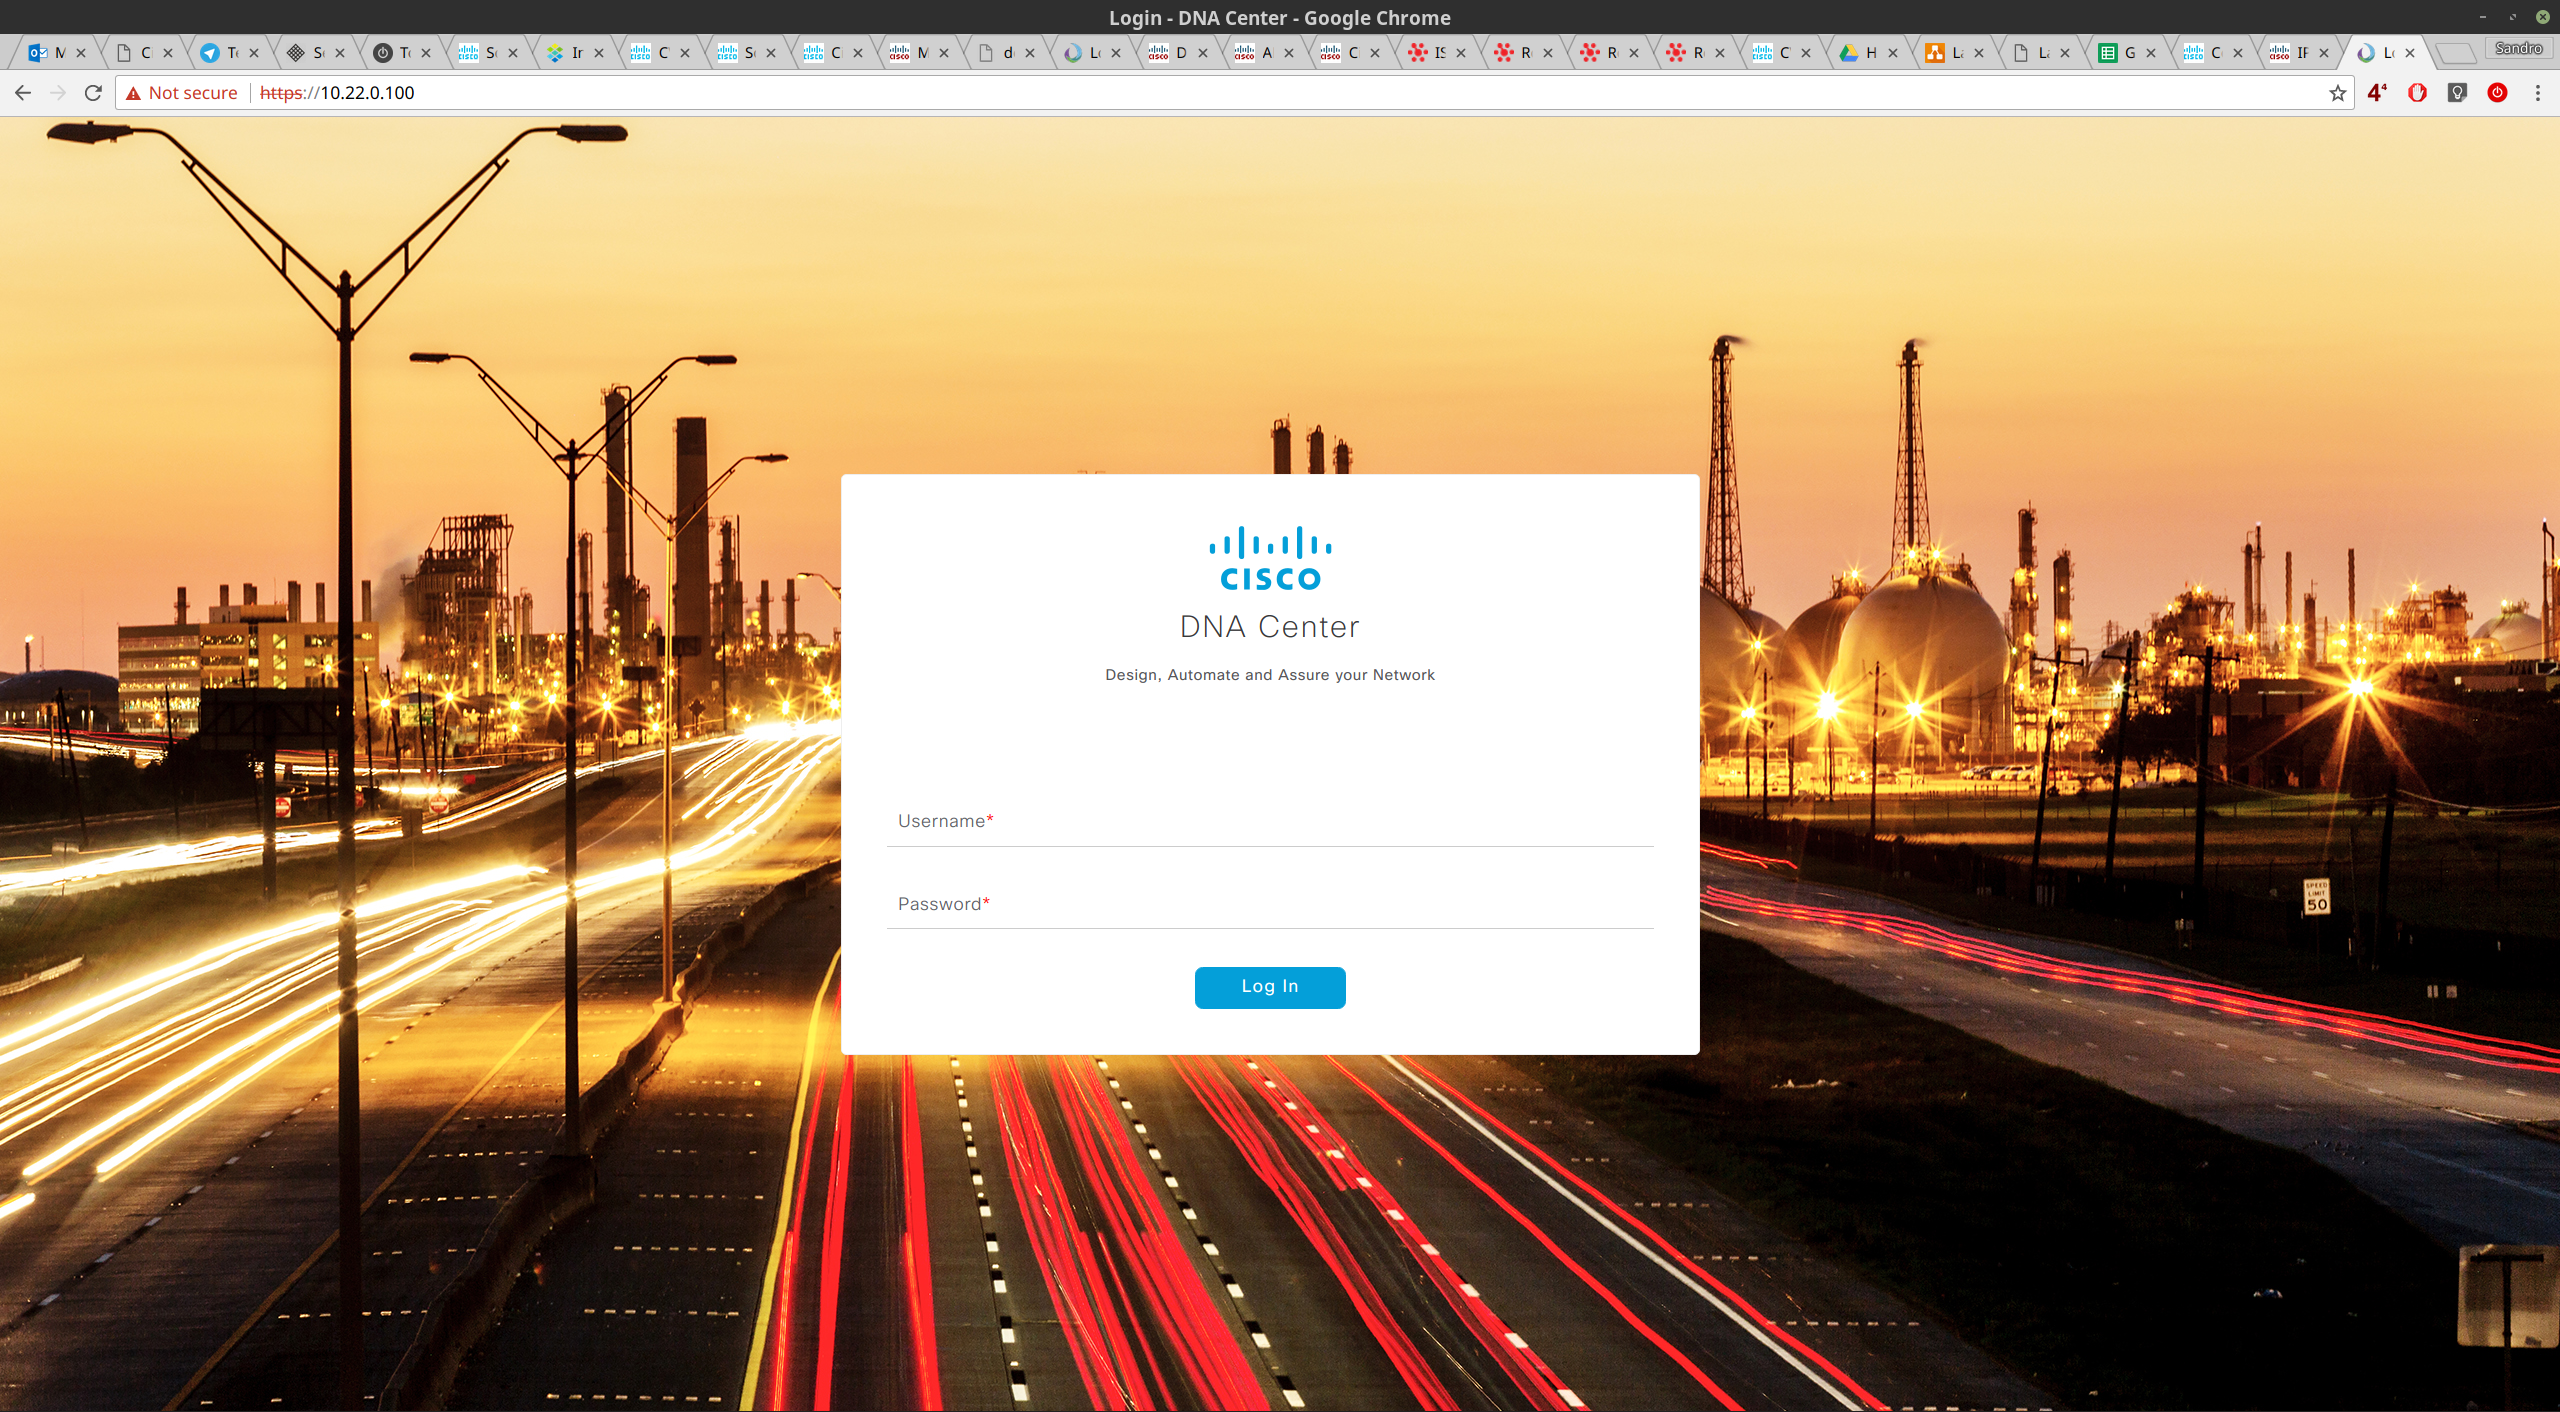
\includegraphics[height=9cm]{img/sc_005.png}
	\caption{DNA Center Web GUI - Loginpage}
	\label{fig:dna-center-gui-1}
\end{figure}

Gleich zu Begin verlangt das DNA Center die Cisco Credentials die mit dem Smart Account verknüpft sind, die die Lizenzen verwaltet. Dieser Schritt kann übersprungen werden. 

\begin{figure}[H]
	\centering
	\includegraphics[height=9cm]{img/sc_006.png}
	\caption{DNA Center Web GUI - Cisco Credentials for Licences}
	\label{fig:dna-center-gui-2}
\end{figure}

Der IPAM Server (in unserem Fall Infoblox) wird auch gleich zu beginn verlangt. Auch dieser Schritt kann vorerst übersprungen werden.

\begin{figure}[H]
	\centering
	\includegraphics[height=9cm]{img/sc_007.png}
	\caption{DNA Center Web GUI - Cisco IPAM}
	\label{fig:dna-center-gui-3}
\end{figure}

\begin{figure}[H]
	\centering
	\includegraphics[height=9cm]{img/sc_008.png}
	\caption{DNA Center Web GUI - Dashboard}
	\label{fig:dna-center-gui-4}
\end{figure}

\subsection{DNA Center Updates}

Der Updateprozess bringt einige Hürden mit sich:
\begin{itemize}
	\item System Updates müssen vor den Package Updates installiert werden.
	\item Werden die Package Updates vor dem System Update ausgeführt, können diese blockieren. 
	\item Die Package Updates müssen in der richten Reihenfolge installiert werden.
	\item Die oben genannte Reihenfolge ist nicht direkt ersichtlich.
	\item Der Updatevorgang dauert mehrere Stunden.
	\item Der Updatefortschritt wird nicht angezeigt. 
	\item Während dem Updateprozess können Teile des Web-GUIs Fehlermeldungen anzeigen oder überhaupt nicht mehr erreichbar sein.
\end{itemize}

Folgende Ansicht ist unter Einstellungen (Zahnrad-Symbol) => Management zu finden:

\begin{figure}[H]
	\centering
	\includegraphics[width=\columnwidth]{img/sc_009.png}
	\caption{DNA Center App Management}
	\label{fig:dna-center-gui-update-1}
\end{figure}

Abgestürzte Packete können mit den folgenden Befehlen wieder restauriert werden (Am Beispiel von main-system-package:1.0.4.779):

\begin{lstlisting}[language=bash]
$ maglev package status | awk  '$3 ~ /[0-9]+/ {print $1":"$3}'| grep -v "^system" |  while read pkg; do maglev catalog package delete $pkg;done
$ maglev system_update_package install main-system-package:1.0.4.779
\end{lstlisting}

Nach einem Update wurde die Reihenfolge von System und Package Update angepasst. Vermutlich um den Administrator dazu zu bringen zuerst die System Updates zu installieren. 

\begin{figure}[H]
	\centering
	\includegraphics[height=4cm]{img/sc_010.png}
	\caption{DNA Center App Management - Alte Menü Anordnung}
	\label{fig:dna-center-gui-update-2}
\end{figure}

\subsubsection{Schwierigkeit: Cisco CCO Login für Updates notwendig}

Application Packages und Updats können nur Installiert werden, wenn die Cisco CCO Credentials hinterlegt sind.

\begin{figure}[H]
	\centering
	\includegraphics[height=4cm]{img/dan-center-cisco-credentials-required.png}
	\caption{DNA Center Upgrade - Cisco Credentials required}
	\label{fig:dna-center-cisco-credentials-required}
\end{figure}

\subsubsection{Schwierigkeit: Unterschiedliche Versionsangabe}

Beim Updatevorgang kann es zu Verwirrungen kommen, weil die Versionangabe von der Funktion About von der Version des System Packages abweicht.

\begin{figure}[H]
	\centering
	\includegraphics[height=3cm]{img/dna-center-about.png}
	\caption{DNA Center - About - Version}
	\label{fig:dna-center-about}
\end{figure}

\begin{figure}[H]
	\centering
	\includegraphics[height=2.5cm]{img/dna-center-system-upgrade-version.png}
	\caption{DNA Center - System Upgrade - Version}
	\label{fig:dna-center-system-upgrade}
\end{figure}

\subsection{Cisco PNP mit DNA Center}

\paragraph{DHCP Konfiguration}

\begin{itemize}
	\item DNA Center akzeptiert Cisco PNP Anfragen via http
	\item Cisco Switches/Router versuchen beim ersten Boot ohne Konfiguration DHCP zu machen und Cisco PNP
\end{itemize}

Die Cisco PNP Discovery kann über die DHCP Optione 43 und 60 konfiguriert werden (Siehe \cite{cisco-pnp-dhcp}). In unserem Fall haben wir diese Optionen auf dem Infoblox konfiguriert.

\begin{figure}[H]
	\centering
	\includegraphics[height=10cm]{img/Infoblox_PNP.png}
	\caption{Infoblox Cisco PNP DHCP Option Konfiguration}
	\label{fig:cisco-pnp}
\end{figure}

\subsection{Automatischer "Claim" von Netzwerkgeräten}

\subsubsection{DNA Center Provision - Unclaimed Devices}

Nachdem die DHCP Option erfolgreich konfiguriert ist, erscheinen die Geräte im Device Inventory.

\begin{figure}[H]
	\centering
	\includegraphics[height=8cm]{img/DNA_Center_All_Fabric2_Unclaimed.PNG}
	\caption{DNA Center Provision - Alle Geräte erfolgreich in der "Unclaimed List"}
	\label{fig:dna-center-provision-unclaimed}
\end{figure}

Bevor es jedoch so weit kam, wurden verschiedene Fehlermeldungen angezeigt. Diese konnten jeweils behoben werden indem das betroffene Gerät auf Werkeinstellung zurückgesetzt und neu gestartet wurde. Dieser Vorgang wurde so lange wiederholt bis keine Fehlermeldungen mehr angezeigt wurden. 

\begin{figure}[H]
	\centering
	\includegraphics[height=4cm]{img/DNA_Center_Unclaimed_Errors_1.PNG}
	\caption{DNA Center Provision - Fehlermeldungen in der "Unclaimed List"}
	\label{fig:dna-center-provision-unclaimed-2}
\end{figure}

\subsection{DNA Center Netzwerk Design}

\subsubsection{Network Hierarchy}

Gemäss unserem \ref{fig:LabNetworkArchitecture} haben wir zwei Standorte. Rapperswil mit zwei Gebäuden und Jona mit einem Gebäude.
In DNA Center können diese sehr einfach im Abschnitt Design => Network Hierarchy hinzugefügt werden.

\begin{figure}[H]
	\centering
	\includegraphics[height=8cm]{img/Selection_011.png}
	\caption{DNA Center Design Map}
	\label{fig:dna-center-design-1}
\end{figure}

\begin{figure}[H]
	\centering
	\includegraphics[height=6cm]{img/Selection_012.png}
	\caption{DNA Center Design - Standort hinzufügen}
	\label{fig:dna-center-design-2}
\end{figure}

\begin{figure}[H]
	\centering
	\includegraphics[height=6cm]{img/Selection_014.png}
	\caption{DNA Center Design - Gebäude können mit Koordinaten hinzugefügt werden.}
	\label{fig:dna-center-design-3}
\end{figure}

\begin{figure}[H]
	\centering
	\includegraphics[height=8cm]{img/design_map_overview.PNG}
	\caption{DNA Center Design - Übersicht über alle Standorte und Gebäude}
	\label{fig:dna-center-design-overview}
\end{figure}

\subsection{Manuelle Underlay Konfiguration mit ISIS}
Da die automatische Erstellung des Underlay Netzwerkes nicht funktionierte, mussten wir es selber Konfigurieren. 

\subsubsection{Script Automation}

\subsubsection{ISIS}

\subsection{Netzwerkgeräte zu Inventory hinzufügen}


\subsection{Manuel Geräte im DNA Center hinzufügen}
Da alle Versuche die Geräte automatisch hinzuzufügen gescheitert sind, entschieden wir uns den Vorgang manuell Durchzuführen. 

Im Dashboard klickt man dazu auf Inventory (Siehe \ref{fig:dna-center-inventory-button})

\begin{figure}[H]
	\centering
	\includegraphics[height=3cm]{img/dna-center-inventory-button.PNG}
	\caption{DNA Center Dashboard - Inventory Knopf}
	\label{fig:dna-center-inventory-button}
\end{figure}

Anschliessend wählt man "Add" (siehe \ref{fig:dna-center-inventory-add})

\begin{figure}[H]
	\centering
	\includegraphics[height=3cm]{img/dna-center-inventory-add.PNG}
	\caption{DNA Center Inventory - Gerät hinzufügen}
	\label{fig:dna-center-inventory-add}
\end{figure}

Anschliessend müssen folgende Informationen eingegeben werden:
\begin{itemize}
	\item Device Type
	\item Device IP \ Name
	\item SNMP (Version, Read und Write Community)
	\item CLI (via SSH oder Telnet) \textit{oder}
	\item NETCONF
\end{itemize}

Wir entschieden uns CLI via SSH zu nehmen. Von NETCONF und CLI muss nur eine von beiden Optionen gewählt werden. 

\begin{figure}[H]
	\centering
	\includegraphics[height=5cm]{img/dna-center-inventory-add-form.png}
	\caption{DNA Center Inventory - Formular Gerät hinzufügen}
	\label{fig:dna-center-inventory-add-form}
\end{figure}

Danach erscheint das Gerät in der Liste (Siehe \ref{fig:dna-center-inventory-index-new})

\begin{figure}[H]
	\centering
	\includegraphics[height=2cm]{img/dna-center-inventory-index-new.png}
	\caption{DNA Center Inventory - Neue Geräte in der Liste}
	\label{fig:dna-center-inventory-index-new}
\end{figure}

TBA: Neue Images herunterladen und mit Golden Tag versehen. 

\subsection{Image Repository}
Im DNA Center können Netzwerkgeräte automatisch geupdatet werden. Sobald ein Gerät im Inventory erfolgreich hinzugefügt worden ist, sucht das DNA Center nach Updates. Die Verfügbaren Images sind unter Desing => Global => Image Repository zu finden.

\begin{figure}[H]
	\centering
	\includegraphics[height=2cm]{img/dna-center-design-image-repository.png}
	\caption{DNA Center Design - Image Respository}
	\label{fig:dna-center-design-image-repository}
\end{figure}

\subsection{Automatisches Softwareupdate von Netzwerkgeräten}

Im DNA Center besteht die Möglichkeit bei "claimed Devices" ein automatisches Softwareupdate durchzuführen. Dies hat bei keinen von unseren Switches oder Routern geklappt. 

\begin{tabular}{ | l | l |}
	\hline
	\textbf{Methode} & \textbf{Resultat} \\
	\hline	
	\makecell{via DNA Center \\ \textit{nutzt HTTP \& SFTP}} & Fehlgeschlagen (Siehe \ref{fig:dna-center-provision-updates-1}) \\
	CLI - HTTPS    & Fehlgeschlagen (Siehe \ref{fig:dna-center-provision-updates-2}) \\
	CLI - SCP      & Fehlgeschlagen (Siehe \ref{fig:dna-center-provision-updates-3}) \\
	CLI - TFTP     & Erfolgreich (Siehe \ref{fig:dna-center-provision-updates-4}) \\	
	\hline	
\end{tabular}
\captionof{table}{Softwareupdate - Übersicht Methoden und ausgeführten Versuche}

\begin{figure}[H]
	\centering
	\includegraphics[height=8cm]{img/updates/Selection_070.png}
	\caption{DNA Center Provision - Nachdem manuellen hinzufügen, muss die Firmware aktualisiert werden.}
	\label{fig:dna-center-provision-updates}
\end{figure}


\begin{figure}[H]
	\centering
	\includegraphics[height=5cm]{img/updates/Selection_071.png}
	\caption{Fehlermeldung Updatevorgang via DNA Center}
	\label{fig:dna-center-provision-updates-1}
\end{figure}

\subsection{Manuelles Softwareupdate via separaten TFTP Server}
Weil das automatische Update nicht funktioniert hat, mussten wir die Images manuell auf die Switches und Router aufspielen.

\begin{figure}[H]
	\centering
	\includegraphics[height=2cm]{img/updates/Selection_082.png}
	\caption{Firmwareupdate Switch via CLI HTTPs}
	\label{fig:dna-center-provision-updates-2}
\end{figure}

\begin{figure}[H]
	\centering
	\includegraphics[height=5cm]{img/updates/Selection_108.png}
	\caption{Firmwareupdate Switch via CLI SCP}
	\label{fig:dna-center-provision-updates-3}
\end{figure}

\begin{figure}[H]
	\centering
	\includegraphics[height=2cm]{img/updates/Selection_111.png}
	\caption{Firmwareupdate Switch via CLI TFTP}
	\label{fig:dna-center-provision-updates-4}
\end{figure}

\subsection{Lizenzen}
Die Lizenzen bezieht das DNA Center automatisch von den Cisco Server. 
\begin{figure}[H]
	\centering
	\includegraphics[height=3cm]{img/LicenceManager_001.png}
	\caption{Der Licence Manager ist über das Dashboard erreichbar.}
	\label{fig:dna-center-licence-1}
\end{figure}

\begin{figure}[H]
	\centering
	\includegraphics[height=6cm]{img/Selection_006.png}
	\caption{Ohne Verlinkten CSSM Account können keine Lizenzen zugewiesen werden.}
	\label{fig:dna-center-licence-3}
\end{figure}

\begin{figure}[H]
	\centering
	\includegraphics[height=6cm]{img/Selection_008.png}
	\caption{Der im DNA Center hinterlegte Cisco Account muss Zugriff zum entsprechenden Smart Account haben.}
	\label{fig:dna-center-licence-4}
\end{figure}

\begin{figure}[H]
	\centering
	\includegraphics[height=5cm]{img/LicenceManager_002.png}
	\caption{Der korrekt hinterlegte Account}
	\label{fig:dna-center-licence-5}
\end{figure}

\begin{figure}[H]
	\centering
	\includegraphics[height=8cm]{img/LicenceManager_003.png}
	\caption{Übersicht über die den Netzwerkkomponeten zugewiesenen Lizenzen}
	\label{fig:dna-center-licence-6}
\end{figure}

\begin{figure}[H]
	\centering
	\includegraphics[height=6cm]{img/LicenceManager_004.png}
	\caption{Nicht jedem Gerät kann eine Lizenz gewiesen werden. (Siehe Tabelle)}
	\label{fig:dna-center-licence-7}
\end{figure}

\begin{tabular}{ | c | c | }
	\textbf{Geräteserie} & 	\textbf{Lizenzzuweisung möglich} \\
	\hline
	Cisco Catalyst 9300 Series Switches & Ja \\
	Cisco Catalyst 3850 Series Ethernet Stackable Switch & Ja \\
	Cisco 4400 Series Integrated Services Routers & Nein \\
\end{tabular}

\subsection{Device Provisioning via DNA Center}
Um den einzelnen Netzwerkgeräten einen Namen und die Basis Konfiguration zu geben, wird im DNA Center unter \textit{Provision -> Devices} die zu provisionierende Geräte ausgewählt. Danach wird \textit{Action -> Provision Device} der Provision Vorgang gestartet.

Dazu muss zuerst im Template Editor ein Template hinzugefügt werden.

TBA: Template Editor Screenshots


\subsection{Overlay Provisioning via DNA Center}


\subsection{BGP über Legacy Netzwerk}

Für das Overlay Provisioning verwendet das DNA Center BGP. Dabei ist uns aufgefallen das die Cisco Catalyst 3850 Series Switche nur eine Lizenz für IP Base installiert haben und BGP nur in der IP Services Lizenz unterstützt wird. Die genauen Unterschiedene der verschiedenen IOS Software Features sind in untenstehender Grafik ersichtlich\cite{cisco-3850-faq}:

\begin{figure}[H]
	\centering
	\includegraphics[width=16cm]{img/IPBaseServices.png}
	\caption{IP Base and Services}
	\label{fig:IP Base and Services}
\end{figure}

Über die CLI konnten konnten wir eine IP Services Evaluation Lizenz für 90 Tage aktivieren.

\begin{lstlisting}[language=bash]
sh license right-to-use activate ipservices all accepptEULA
reload
show license right-to-use
\end{lstlisting}

\subsection{Fabric Konfigurieren}
Nach der manuellen Konfiguration des Underlays, dem hinzufügen der Geräte, dem Update und dem Provisionieren, konnten wir endlich die Fabric konfigurieren. 

Erreichbar ist das unter \textit{Provision -> Fabric}. Nachfolgend wir der entsprechende Standort ausgewählt.

Den einzelnen Netzwerkgeräten werden nun mit Rechtsklick folgende Rollen zugeteilt:
\begin{itemize}
	\item Border
	\item Border + CP (Control Plane)
	\item Edge
\end{itemize}

Nachdem alle Geräte der entsprechenden Fabric zugeteilt worden sind, kann die Konfiguration gespeichert und wird auf die Geräte geschrieben. 

\begin{figure}[H]
	\centering
	\includegraphics[width=16cm]{img/dna-center-fabric-1.png}
	\caption{DNA Center Provision - Fabric - Nach der Zuteilung wird die Konfiguration auf die Geräte geschrieben.}
	\label{fig:IP Base and Services}
\end{figure}


\begin{tabular}{| l | l | l | l | l |}
	\textbf{Darstellung} & \makecell{\textbf{Teil der}\\ \textbf{Fabric}} & \makecell{\textbf{Änderung}\\ \textbf{ausstehend}} & \textbf{Provisioniert} & \textbf{Bemerkung} \\
	\hline
	Grau & Ja & Nein & Nein & \\
	Schwarz & Nein & Nein & Nein & \\
	Grau mit blauem Rand & Ja & Ja & Nein & \\
	Blau & Ja & Nein & Ja & \\
	Umrandung mit Pfeil & - & - & - & Gruppierte Geräte\\	

\end{tabular}
\captionof{table}{DNA Center Provision - Fabric - Darstellung}

\subsection{Policies definieren}
Damit die Fabric Konfiguriert werden kann, müssen folgende Bedienungen erfüllt sein:





\subsection{Cisco ISE Verknüpfen und Gruppen anlegen}

\subsection{Ping zwischen zwei Clients}

\subsection{DNA Center Reset}
Da nach einigen Versuchen weder ein funktionsfähiges Under- noch Overlay Netzwerk vorhanden war, hatten wir uns entschieden das DNA Center neu zu Konfigurieren.

\begin{lstlisting}[language=bash]
$ maglev-config-wizard #DO NOT EXECUTE THIS COMMAND
\end{lstlisting}

Als folge dieses Befehls, nachdem alle Parameter eingegeben wurden, kam die folgende Meldung:

\begin{figure}[H]
	\centering
	\includegraphics[height=10cm]{img/dna-center-reset-fail-1.png}
	\caption{DNA Center - maglev-config-wizard - Fehlermeldung}
	\label{fig:dna-center-reset-1}
\end{figure}

Nach einem Neustart der Appliance kam die folgende Meldung und das System bootete nicht mehr. 
\begin{figure}[H]
	\centering
	\includegraphics[height=1cm]{img/dna-center-reset-fail-2.png}
	\caption{DNA Center - Boot Fehlermeldung}
	\label{fig:dna-center-reset-2}
\end{figure}

In der Anleitung wird dieser Befehl so nicht erwähnt. Bei einem früheren Versuch diesen Befehl auszuführen, um den NTP Server zu ändern, führte es jedoch nicht zu diesem Fehler. 

\paragraph{Neuinstallation}
In folge war es notwendig die Cisco DNA Center Appliance neu zu installieren. 

\begin{figure}[H]
	\centering
	\includegraphics[height=2cm]{img/dna-center-reset-iso.png}
	\caption{DNA Center - Neuinstallation - Installations ISO wird auf USB Drive kopiert}
	\label{fig:dna-center-iso-1}
\end{figure}

Das USB Drive wird direkt in die Appliance gesteckt und gebootet. Der weitere Installationsprozess sieht aus wie im Abschnitt \ref{DNACenterSetup_Installation} gezeigt. 

\alertwarningbox{
	Nach der Neuinstallation sind alle Daten und die Konfiguration gelöscht. Eine Option die Konfiguration beizubehalten gibt es nicht.
}

\subsection{Zweiter Versuch}
Im ersten Versuch haben wir die LAN Automation übersprungen. Das stellt jedoch einer der wichtigen Features des DNA Centers dar. Mit der Unterstützung von Patrick Mosimann sind wir alles Schritt für Schritt durchgegangen. 

\subsection{DNA Center Netzwerk Design}
Wie im ersten Teil

\subsection{Alle Netzwerkkomponenten vorgehen}

\subsection{ISE reset}

\subsection{Credentials korrekt hinterlegen}

\subsection{Fabric Border - Seeddevice}

\subsection{ISE Integration}

\subsection{Netzwork Discovery - LAN Automation}


\section{Ergebnisdiskussion}
Stärken und Schwächen der Konzepte, Verbesserungen für die Zielgruppe im Kontext




Zur Zeit läuft nur die Rapperswil Seite. Jona wurde noch nicht implementiert, um zuerst auf der Seite von Rapperswil eine laufende Fabric mit Policies zu erstellen.

Eventuell af Traces verweisen was wie funktioniert hat.

Bugs und eventuell noch ausstehende Antworten auf Fragen erwähnen

Verbesserungen in Bezug auf vorhandene Bugs und unsere Grafik in Vorgehen mit Schwierigkeiten


\section{Schlussfolgerungen}

\subsection{Erreichte Ziele}
Zusätzlich zum Ziel das Netzwerk mit Underlay und Overlay aufzusetzen, konnten alle Use Cases praktisch oder theoretisch in der Arbeit abgedeckt werden. 
\subsection{Mögliche Verbesserungen}
Um noch mehr Netzwerkorchestrierung über Programmierschnittstellen zu erreichen sind die kommenden Erweiterungen der API des Cisco DNA Centers unabdingbar. Die in dieser Arbeit bisher aufgetretenen Bugs, sind für eine neue und moderne Software nicht ungewöhnlich, müssen in zukünftigen Releases aber behoben werden.
 
\subsection{Zukunft}
Die Verwaltung des Netzwerkes durch einen zentralen Controller, wie das Cisco DNA Center, schafft viel Vorteile. In der Zukunft können sich Netzwerkingenieure mehr auf ertragreiche Aufgaben, wie das Netzwerkdesign und die Überwachung, konzentrieren. Dank des vereinfachten und zentralen Troubleshootings mit der Cisco DNA Center Assurance sind Netzwerkprobleme im Handumdrehen gelöst. Des Weiteren bietet die API in den kommenden Versionen des Cisco DNA Centers die Möglichkeit alle Netzwerkgeräte über eine einzige Schnittstelle zu programmieren und an externe Systeme anzubinden. Der komplexe und aufwändige Zugriff auf jedes einzelne Gerät entfällt. 
\section{Abkürzungsverzeichnis}
\begin{acronym}[SEPSEPSEP]
	\acro{AAA}{authentication, authorization, and accounting}
	\acro{ACI}{Application Centric Infrastructure}
	\acro{ACL}{access control list}
	\acro{AP}{access point}
	\acro{API}{application programming interface}
	\acro{BGP}{border gateway protocol}
	\acro{CAPWAP}{control and provisioning of wireless access points protocol}
	\acro{CCO}{Cisco Connection On-line}
	\acro{CMD}{Cisco Meta Data}
	\acro{DMVPN}{Dynamic Multipoint VPN}
	\acro{DNA}{Cisco Digital Network Architecture}
	\acro{EID}{Endpoint Identifier}
	\acro{GRE}{Generic Routing Encapsulation}
	\acro{GUI}{Graphical User Interface}
	\acro{GW}{Gateway}
	\acro{HTDB}{Host Tracking Database}
	\acro{IGP}{Interior Gateway Protocol}
	\acro{IP}{Internet Protocol}
	\acro{IPAM}{IP-Adress-Management}
	\acro{ISE}{Cisco Identity Services Engine}
	\acro{LAN}{Local Area Network}
	\acro{LISP}{Locator/ID Separation Protocol}
	\acro{MPLS}{Multiprotocol Label Switching}
	\acro{MR}{Map Resolver}
	\acro{MS}{Map Server}
	\acro{MTU}{Maximum Transmission Unit }
	\acro{PnP}{Plug and Play}
	\acro{RLOC}{Routing locator}
	\acro{SDA}{Software-Defined Access}
	\acro{SDN}{Software-Defined Networking}
	\acro{SGACL}{Scalable Group Access Control List}
	\acro{SGT}{Scalable Group Tag}
	\acro{SXP}{Scalable Group Tag Exchange Protocol}
	\acro{VLAN}{Virtual Local Area Network}
	\acro{VN}{Virtual Network}
	\acro{VNI}{Virtual Extensible LAN Network Identifier}
	\acro{VPN}{Virtual Private Network}
	\acro{VRF}{Virtual Routing and Forwarding}
	\acro{VTEP}{Virtual Extensible LAN Tunnel Endpoint}
	\acro{VXLAN}{Virtual Extensible LAN}
	\acro{WAN}{Wide Area Network}
	\acro{WLAN}{Wireless Local Area Network}
\end{acronym}

%\ac{Kuerzel} Bei der ersten Verwendung von \ac{Kuerzel} wird die Langfassung der Abkürzung und die Abkürzung selbst in Klammern dargestellt. Wird der Befehl \ac{Kuerzel} das nächste mal aufgerufen erschneit nur nocht die Abkürzung.

%\acf{Kuerzel} Mit \acf{Kuerzel} gibt es ein zweites Erstes Mal für diese Abkürzung. Das heißt, sie wird wieder in der Langform und der geklammerten Abkürzung gezeigt.

%\acs{Kuerzel} \acs{Kuerzel} gibt nur die Abkürzung aus.

%\acl{Kuerzel} \acl{Kuerzel} gibt nur die Langform der Abkürzung aus.







\newpage
\appendix
\pagenumbering{Roman}

\section{Installationsanleitung}

\subsection{DNA Center Setup}



\subsubsection{DNA Center Reset}



\subsection{DNA Center Network Discovery}

Um die Netzwerkkomponenten zum DNA Center hinzuzufügen, wurde mehrere Versuche unternommen. 

\section{Benutzerhandbuch}

\subsection{Updates}
Es ist wichtig das DNA Center auf einem aktuellen Stand zu halten, da sehr häufig neue Updates publiziert werden.

Auf folgender Webseite veröffentlicht Cisco die Sicherheitslücken und erklärt gleich zu welcher Version das DNA Center geupdatet werden muss:
\url{https://tools.cisco.com/security/center/publicationListing.x?resourceIDs=233151\&apply=1\&totalbox=1\&pt0=Cisco\&cp0=233151\#~FilterByProduct}

\subsubsection{Updates installieren}
\begin{enumerate}
	\item Ausgehend vom DNA Center Dashboard nach \textit{Settings $\rightarrow$ System Settings $\rightarrow$ App Management} navigieren
	\item Das gewünschte System Update oder Package markieren und mittels \textit{Action $\rightarrow$ Download} herunterladen
	\item Das heruntergeladene Update markieren und mittels \textit{Action $\rightarrow$ Install} installieren
\end{enumerate}

Es ist zu beachten, dass System Updates immer vor den Package Updates installiert werden müssen. Des Weiteren sollen die restlichen Funktionen des DNA Centers während dem Update nicht verwendet werden.

\subsection{Design}
Mit dem Design wird die physische Struktur bis auf die Gebäude genau hinterlegt. Zusätzlich werden Informationen hinterlegt, die das DNA Center während der Provisionierung auf die Netzwerkkomponenten schreibt.

\subsubsection{Site hinzufügen}
\begin{enumerate}
	\item Ausgehend vom DNA Center Dashboard nach \textit{Design $\rightarrow$ Network Hierarchy} navigieren
	\item \textit{Add Site} wählen
	\item Im neuen Popup den gewünschten Namen eingeben
	\item \textit{Add} anwählen
\end{enumerate}

\subsubsection{Gebäude zur Site hinzufügen}
\begin{enumerate}
	\item Ausgehend vom DNA Center Dashboard nach \textit{Design $\rightarrow$ Network Hierarchy} navigieren
	\item \textit{Add Site} wählen
	\item Im neuen Popup den gewünschten Namen eingeben
	\item \textit{Building} anwählen
	\item Adresse und/oder Koordinaten eingeben
	\item \textit{Add} anwählen.
\end{enumerate}


\subsubsection{Netzwerkdienste Konfigurieren}
\begin{enumerate}
	\item Ausgehend vom DNA Center Dashboard nach \textit{Design $\rightarrow$ Network Settings} navigieren. 
	\item \textit{Global} wählen
	\item Bei \textit{AAA Server Network} und \textit{Client/Endpoint} anwählen
	\item Bei \textit{Network $\rightarrow$ ISE} wählen und entsprechende IP Adresse eingeben
	\item Bei \textit{Network $\rightarrow$ RADIUS} wählen und entsprechende IP Adresse eingeben
	\item Bei \textit{Client/Endpoint $\rightarrow$ Servers $\rightarrow$ ISE} wählen und entsprechende IP Adresse eingeben
	\item Bei \textit{Client/Endpoint $\rightarrow$ Protocol $\rightarrow$ RADIUS} wählen und entsprechende IP Adresse eingeben
	\item Bei \textit{DHCP Server} das \textbf{PLUS}-Zeichen anklicken und die IP Adresse des DHCP Servers hinterlegen 
	\item \textit{SYSLOG Server}, \textit{SNMP Server} und \textit{Netflow Collector Server} können leer gelassen werden
	\item Mit einem Klick auf \textit{Save} ist alles abzuspeichern
\end{enumerate}

\subsubsection{Device Credentials hinterlegen}
\begin{enumerate}
	\item Ausgehend vom DNA Center Dashboard nach \textit{Design $\rightarrow$ Network Settings $\rightarrow$ Device Credentials} navigieren
	\item \textit{Add} wählen
	\item \textit{Name}, \textit{Username}, \textit{Password} und \textit{Enable Password} eingeben
	\item Mit einem Klick auf \textit{Save} alles abspeichern
\end{enumerate}

\subsubsection{IP Address Pools hinzufügen}
Das DNA Center benötigt verschiedene IP Adressen Pools. Die Grösse der Pools ist entsprechend der Anforderungen in der Umgebung zu wählen.
\begin{itemize}
	\item Ein Pool für die LAN Automation (P2P Links, Loopback Adressen)
	\item Ein Pool für die Border Konfiguration
	\item Für jedes VN ein Pool
\end{itemize}

Weitere Pools können jederzeit hinzugefügt werden.

\begin{enumerate}
	\item Ausgehend vom DNA Center Dashboard nach \textit{Design $\rightarrow$ Network Settings $\rightarrow$ IP Address Pools} navigieren
	\item \textit{Add IP Pool} wählen
	\item Nun gilt es einen IP Pool Name, ein IP Subnet, ein CIDR Präfix, eine Gateway IP Adresse einzugeben
	\item Der korrekte DHCP Server und DNS Server ist per Dropdown auszuwählen
	\item Mit einem Klick auf \textit{Save} die Eingaben speichern
\end{enumerate}

\subsubsection{Templates erstellen}
Um Konfigurationen auf den Geräten vorzunehmen, die nicht vom DNA Center abgedeckt sind, können Templates definiert werden.
\begin{enumerate}
	\item Ausgehend vom DNA Center Dashboard nach \textit{Template Editor navigieren}
	\item \textbf{PLUS} Zeichen anwählen und \textit{Add Project} wählen
	\subitem Einen Namen für das Projekt angeben und speichern
	\item \textbf{PLUS} Zeichen anwählen und \textit{Add Template} wählen
	\item \textit{Name, Projekt, Device Type und Software Type} wählen und speichern
	\item Im Editor die gewünschte Konfiguration eingeben
	\item Template mittels \textit{Actions $\rightarrow$ Save} und \textit{Actions $\rightarrow$ Save} speichern
\end{enumerate}

\subsubsection{Netzwerkprofile erstellen}
Um die erstellten Templates anwenden zu können, müssen Netzwerkprofile erstellt werden.
\begin{enumerate}
	\item Ausgehend vom DNA Center Dashboard nach \textit{Design $\rightarrow$ Network Profiles} navigieren
	\item \textit{Add Profile} klicken und \textit{Switching Profile} wählen
	\item \textit{Name} definieren
	\item Mittels \textit{Add} die gewünschten Templates hinzufügen
\end{enumerate}

\subsubsection{Netzwerkprofile zuweisen}
Damit die Netzwerkprofile angewendet werden, müssen diese noch den nötigen Sites zugewiesen werden.
\begin{enumerate}
	\item Ausgehend vom DNA Center Dashboard nach \textit{Design $\rightarrow$ Network Profiles} navigieren
	\item In der Zeile des gewünschten Profils auf \textit{Sites} klicken
	\item Im neuen Popup alle nötigen Sites über das Multidropdown-Menü hinzufügen
	\item Mit \textit{Save} das Netzwerkprofil speichern
\end{enumerate}

\subsection{Policies}

\subsubsection{Virtual Network}
Virtuelle Netzwerke dienen der Isolierung der Netzwerkbenutzer und dienen somit der Sicherheit. Standardmässig können Hosts in unterschiedlichen virtuellen Netzwerken nicht miteinander kommunizieren. Mit Hilfe von virtuellen Netzwerken kann das physische Netzwerk in mehrere logische Netzwerk geteilt werden. Ein typischer Anwendungsfall ist die Segmentierung von Gästen, Mitarbeitern und Kontraktor in getrennte Gruppen, so dass der Zugriff nur auf Teile des Netzwerkes erlaubt oder eingeschränkt werden kann. Die verschiedenen Arten von Netzwerken sind:

\begin{itemize}
	\item Gast-Netzwerk: Netzwerkverbindungen, die von einem Unternehmen zur Verfügung gestellt werden, um seinen Gästen den Zugang zum Internet und zum eigenen Unternehmen zu ermöglichen, ohne die Sicherheit der Unternehmens Infrastruktur zu beeinträchtigen. Gäste können auf das Internet zugreifen, aber nicht auf interne Anwendungen.
	\item Mitarbeiter-Netzwerk: Netzwerkverbindungen, die den Zugriff auf das Internet und interne Anwendungen ermöglichen. Diese Gruppe kann weiter segmentiert werden, um Zugriffe innerhalb des Firmennetzwerks zu regeln und für spezifische Benutzer und Gruppen einzuschränken.
	\item Kontraktor-Netzwerk: Netzwerkverbindung, die es den Benutzern ermöglicht, auf das Internet und auf unternehmensspezifische Anwendungen innerhalb des Unternehmensnetzwerks zuzugreifen. 
\end{itemize}

\subsubsection{Virtual Network hinzufügen}
\begin{enumerate}
	\item Ausgehend vom DNA Center Dashboard nach \textit{Policy $\rightarrow$ Virtual Network} navigieren.
	\item \textbf{PLUS} Zeichen anwählen
	\item \textit{Virtual Network Name} eingeben
	\item Scalable Groups per Drap\&Drop in das Virtual Network ziehen
	\item Mit \textit{Save} speichern
\end{enumerate}

\subsubsection{Scalable Group}
Scalable Groups umfassen eine Gruppierung von Benutzern, Endgeräten oder Ressourcen, die dieselben Anforderungen an die Zugriffskontrolle stellen. Diese Gruppen, in Cisco ISE als Sicherheitsgruppen oder SGs bekannt, werden auf dem Cisco ISE definiert. 

\paragraph{Scalable Group hinzufügen}
\begin{enumerate}
	\item Ausgehend vom DNA Center Dashboard nach \textit{Policy $\rightarrow$ Registry $\rightarrow$ Scalable Groups} navigieren
	\item \textit{Add Groups} wählen
	\item In Cisco ISE einloggen
	\item \textit{+ Add} anklicken
	\item \textit{Name, Icon und Beschreibung} eingeben 
	\item Mit \textit{Submit} speichern
\end{enumerate}
Die erstellte Scalable Group ist nun auch im DNA Center verfügbar und kann verwendet werden um Policies zu definieren.

\subsubsection{Access Control Contract}
Ein Zugriffsvertrag ist eine Security Group Access Control List (SGACL). Sie definiert das Regelwerk, dass die Netzwerkinteraktion zwischen Quelle und Ziel in einer Zugriffskontrollrichtlinie regelt.

\subsubsection{Group-based Access Control Policy}
Gruppenbasierte Zugriffskontrollrichtlinien sind Security Group Access Control Lists (SGACLs). DNA Center hat den Cisco ISE integriert, um den Prozess der Erstellung und Pflege von SGACLs zu vereinfachen. Während der initialen Integration von DNA Center und Cisco ISE werden skalierbare Gruppen und Richtlinien, die in Cisco ISE vorhanden sind, an das DNA Center weitergegeben und in das standardmäßige virtuelle Netzwerk eingefügt.

Das folgende Beispiel zeigt den Prozess der Authentifizierung und Zugriffskontrolle, den ein Benutzer durchläuft, wenn er sich in das Netzwerk einloggt:
\begin{enumerate}
	\item Ein Benutzer verbindet sich mit einem Port auf einem Switch und stellt seine Zugangsdaten zur Verfügung.
	\item Der Switch kontaktiert Cisco ISE.
	\item Cisco ISE authentifiziert den Benutzer und lädt die SGACLs auf den Port, mit dem der Benutzer verbunden ist.
	\item  Dem Benutzer wird der Zugang zu bestimmten Benutzern oder Geräten (Servern) auf der Grundlage des in die SGACL gewährt.
\end{enumerate}

\subsubsection{Workflow}
Workflow zur Konfiguration einer gruppenbasierten Zugriffskontrollrichtlinie.

\begin{table}[H]
	\rowcolors{2}{gray!25}{white}
	\centering
	\begin{tabularx}{\textwidth}{p{2 cm} | X | p{2 cm}}
		\rowcolor{gray!50}
		\textbf{Schritt} & \textbf{Aktion} & \textbf{Zweck} \\
		\hline	
		1 & Erstellen eines virtuellen Netzwerkes. Abhängig von der Konfiguration des Unternehmens und seinen Zugriffsanforderungen und -beschränkungen können die Gruppen in verschiedene virtuelle Netzwerke unterteilt werden, um eine weitere Segmentierung zu ermöglichen. & (Optional) \\
		2 & Erstellen einer skalierbaren Gruppe. Nach der Integration von Cisco ISE werden die in ISE vorhandenen skalierbaren Gruppen in das DNA Center übertragen. Wenn eine skalierbare Gruppe nicht besteht, kann diese direkt angelegt werden. & (Optional) \\
		3 & Erstellen eines Zugriffskontrollvertrag (access control contract). Ein Contract definiert eine Reihe von Regeln, die eine Aktion (erlauben oder verweigern), die Netzwerkgeräte basierend auf dem Datenverkehr durchführen, der bestimmten Protokollen oder Ports entspricht. & \\
		4 & Erstellen einer gruppenbasierten Zugriffskontrollrichtlinie (group-based access control policy). Die Zugriffskontrollrichtlinie definiert den Zugriffskontrollvertrag, der den Verkehr zwischen den skalierbaren Quell- und Zielgruppen regelt. & \\
		
	\end{tabularx}
	\caption{Workflow zur Erstellung der Access Control Policies}
	\label{tab:Workflow zur Erstellung der Access Control Policies}
\end{table}

\subsection{Erstellen einer Group-Based Access Control (Fabric)}
\begin{enumerate}
	\item Wähle auf der DNA Center Homepage \textit{Policy $\rightarrow$ Contracts $\rightarrow$ Access Contracts}.
	\item Klick \textit{Add Contract}.
	\item Im Dialogfenster des \textit{Contract Editor} kann ein Namen und eine Beschreibung für den Vertrag erfasst werden.
	\item Wähle in der Dropdown-Liste \textit{Implicit Action} entweder \textit{Deny} oder \textit{Permit}.
	\item Wähle aus der Dropdown-Lste in der Spalte \textit{Port/Protocol} einen Port oder ein Protokoll aus. Hinweis: Wenn das DNA Center nicht über den Port oder das Protokoll verfügt welches benötigt wird, kann dies selbst erstellt werden. Klicke hierzu auf \textit{Add Port/Protocol}, füge alle erforderlichen Informationen hinzu und klicke auf \textit{Save}.
	\item (Optional) Um weitere Regeln in den Vertrag aufzunehmen, klicke auf \textit{Add} und wiederhole Schritt 5 und 6.
	\item Klicke \textit{Save}.
\end{enumerate}

\subsection{Provision}
\subsubsection{Seed Device manuell konfigurieren}

\subsubsection{LAN Automation durchführen}

\subsubsection{Netzwerkkomponenten Provisionieren}

\subsubsection{Fabric erstellen}
\paragraph{Border + CP festlegen}
\paragraph{Intermediate Nodes festlegen}
\paragraph{Edge Nodes festlegen}

\subsubsection{Host Onboarding}

\paragraph{Virtual Networks auswählen}
~\\
Um ein Virtual Network verwenden zu können, muss dieses in der entsprechenden Fabric zuerst aktiviert und ein IP Pool zugewiesen werden. 
\begin{enumerate}
	\item Ausgehend vom DNA Center Dashboard nach \textit{Provision $\rightarrow$ Fabric $\rightarrow$ FABRIC\_NAME $\rightarrow$ Host Onboarding} navigieren. 
	\item Im Abschnitt \textit{Virtual Networks} werden nun alle gewünschten \textit{Virtual Networks} ausgewählt. 
	\item Im neuen Popup wird der gewünschte IP Pool ausgewählt. 
	\item Der Dialog wird mit einem Klick auf \textit{Update} geschlossen.
\end{enumerate}


\paragraph{Ports konfigurieren}
~\\
Für jeden Port, der nicht bereits für die Konnektivität zwischen den Fabric Nodes verwendet wird, kann ein Addresspool, eine Gruppe und eine Authentifizierungsmethode (Siehe: \ref{authentifizierungsmethoden}) definiert werden. 
\begin{enumerate}
	\item Ausgehend vom DNA Center Dashboard nach \textit{Provision $\rightarrow$ Fabric $\rightarrow$ FABRIC\_NAME $\rightarrow$ Host Onboarding} navigieren. 
	\item Im \textit{Select Port Assignment} werden die zu konfigurierende Ports \textit{Virtual Networks} ausgewählt. 
	\item Für die ausgewählten Ports wird nun ein \textit{Address Pool}, \textit{Scalable Group}, \textit{Voice Pool} und eine Authentifizierungsmethode gewählt. 
	\item Die Änderungen werden mit einem Klick auf \textit{Save} gespeichert. 
\end{enumerate}




\section{Projektmanagement}

\subsection{Projektübersicht}
Das Hauptziel dieser Studienarbeit ist die Installation des DNA Centers und Integration eines Campus Labor Netzwerkes.

\subsubsection{Ziele der Projektes}
Da SDN im Campus Bereich Neuland ist, soll die SDA Lösung vom Hersteller Cisco ausgearbeitet werden. Dazu gehören folgende Ziele:

\begin{itemize}
	\item Installation von DNA Center und Integration vom Campus Labor Netzwerk
	\item Definition von Benutzer- und Geräteprofilen, um basierend auf Geschäftsanforderungen die Zugriffsrechte und Netzwerksegmentierung zu verwalten und so das Netzwerk sicher zu halten
	\item Verwendung von Erkenntnissen von DNA Analytics and Assurance für eine proaktive Überwachung, Fehlerbehebung und Optimierung des Netzwerks
	\item Integration vom bestehendem IPAM Tool im DNA Center
	\item Erstellung von wöchentlichen Reports über den Campus Netzwerk Status in einem E-Mail 
\end{itemize}

\subsection{Projektorganisation}
Diese Studienarbeit wird von drei Personen umgesetzt und durch zwei Betreuer überwacht.

\subsubsection{Organisationsstruktur}
\begin{figure}[H]
	\centering
	\includegraphics[height=5cm]{img/Organisationsstruktur.png}
	\caption{Organisationsstruktur}
	\label{fig:Organisationsstruktur}
\end{figure}

\subsection{Management Abläufe}
Für die Umsetzung der Studienarbeit stehen insgesamt 15 Wochen und pro Person 240 Stunden zur Verfügung. In einer Woche liegt das Arbeitspensum von 16 Stunden pro Person vor. Das Projekt startet am 19. Februar 2018 und endet am 15. Juni 2018.

\subsubsection{Zeitliche Planung}
Die zeitliche Planung, sowie die Verwaltung der Arbeitspakete erfolgte auf Waffle.io. Die Planung wird während dem Projekt laufend aktualisiert und angepasst. Die Arbeitszeiten werden während der Arbeitsausführung mit Toggle erfasst.

\begin{figure}[H]
	\centering
	\includegraphics[width=16cm]{img/ZeitlichePlanung_v4.png}
	\caption{Projektplanung}
	\label{fig:Projektplanung}
\end{figure} 

\subsubsection{Meilensteine}
Folgende Meilensteine sind für das Projekt definiert:
\begin{table}[H]
	\rowcolors{2}{gray!25}{white}
	\centering
	\begin{tabularx}{\textwidth}{p{1cm}| p{2.5cm}| X}
		\rowcolor{gray!50}
		\textbf{Nr} & \textbf{Datum} & \textbf{Meilenstein} \\
		\hline	
		M0 & 27.02.2018 & Kickoff Meeting \\
		M1 & 10.04.2018 & Projektplanung abgeschlossen \\
		M2 & 24.04.2018 & Inbetriebnahme Hardware abgeschlossen \\
		& 16.05.2018 & Zwischenpräsentation \\
		M3 & 01.06.2018 & Fabric Konfiguration \\
		M4 & 10.06.2018 & Definierung von Benutzer- und Geräteprofilen \\
		M5 & 12.06.2018 & Reporting und Monitoring \\
		M6 & 13.06.2018 & Freigabe des Abstracts \\
		M7 & 13.06.2018 & Abgabe Projekt \\
		& 15.06.2018 & Endpräsentation \\
	\end{tabularx}
	\caption{Meilensteine}
	\label{tab:Meilensteine}
\end{table}


\subsubsection{Arbeitspakete}
Alle Arbeitspakete werden in Waffle.io erfasst und sind unter folgendem Link ersichtlich:
\href{Waffle.io}{https://waffle.io/night28/HSR\_SA}
\subsubsection{Besprechungen}
Die Besprechungen mit dem Betreuer finden an den nachfolgend aufgelisteten Tagen statt:
\begin{itemize}
	\item jeden Dienstag zwischen 15.10 - 16.10 Uhr
\end{itemize}

Offene Traktanden und Probleme werden mit dem Betreuer diskutiert. Nach dieser Besprechung wird jeweils in einem Team-Meeting das weitere Vorgehen geplant.


\subsection{Infrastruktur}
Die Organisation der Arbeit und Teammitglieder wird durch folgende Werkzeuge unterstützt:

\begin{figure}[H]
	\centering
	\includegraphics[width=13cm]{img/EingesetzteToolsZurOrganisation.png}
	\caption{Übersicht über die Verknüpfung der eingesetzten Werkzeuge zur internen Organisation.}
	\label{fig:Interne Organisationsstruktur}
\end{figure} 

Unsere Tools sind unter folgenden Links einsehbar:
\paragraph{GitHub} \href{https://github.com/night28/HSR_SA}{https://github.com/night28/HSR\_SA} 

\paragraph{Waffle.io} \href{https://waffle.io/night28/HSR\_SA}{https://waffle.io/night28/HSR\_SA}

\paragraph{Toggl} \href{https://toggl.com/}{https://toggl.com/}
 
\subsection{Risiko Management}

\subsubsection{Umgang mit Risiken}

Risiken lassen sich nicht vermeiden. Aus diesem Grund sind nachfolgend mögliche Risiken aufgeführt. Des Weiteren wurden vorbeugende Massnahmen definiert, um die Eintrittswahrscheinlichkeit von Risiken mit schwerwiegenden Konsequenzen zu reduzieren. Für den Fall, dass ein Risiko dennoch eintreten sollte, sind entsprechende Massnahmen definiert, um den Schaden möglichst gering zu halten.
Sollten sich während dem Projekt neue potenzielle Risiken zeigen, wird dieses Dokument laufend aktualisiert.

\begin{landscape}

\subsubsection{Risiken}
\newcommand*\rot{\rotatebox{90}}
\rowcolors{2}{gray!25}{white}
\begin{longtable}{|m{0.5cm}|m{3cm}|m{5cm}|m{0.75cm}|m{0.75cm}|m{0.75cm}|m{5cm}|m{5cm}|} 
	\hline
	\rot{Nummer} & \rot{Titel} & \rot{Beschreibung} & \rot{\shortstack[l]{maximaler\\Schaden [h]}} & \rot{\shortstack[l]{Eintritts-\\wahrscheinlichkeit}} & \rot{\shortstack[l]{Gewichteter\\Schaden [h]}} & \rot{Vorbeugung} & \rot{\shortstack[l]{Verhalten beim\\Eintreten}} \\
	\hline\hline
	1 & Ausfall eines Teammitglieds & Ausfall auf Grund unvorhergesehener Ereignisse wie Krankheit, Unfall etc. & 40 & 15\% & 6 & Reserven einplanen, Kommunikation sicherstellen, damit andere Teammitglieder die Aufgaben übernehmen können & Tasks des ausgefallen Mitglieds möglichst auf die anderen Teammitglieder aufteilen. \\ 
	\hline
	2 & Hardwareausfall DNA-Center & DNA-Center Appliance fällt durch Hardwaredefekt aus & 30 & 5\% & 1.5 & keine vorbeugenden Massnahmen möglich & Austausch im Rahmen der Garantie veranlassen \\
	\hline
	3 & Fehlendes Know-How & Da viele der Themen neu sind, kann entsprechendes Wissen fehlen & 40 & 20\% & 8 & Zeit einplanen, um sich in neue Themen einzuarbeiten & Fehlendes Wissen sobald wie möglich aneignen. Bei Bedarf Rat der Betreuer einholen \\
	\hline
	4 & Konflikte oder Missverständnisse im Team & Das Team ist sich bezüglich wichtigen Entscheidungen uneinig & 25 & 15\% & 3.75 & Entscheidungen stets mit Begründung dokumentieren & Kann auch mit Hilfe der Dokumentation keine Einigung gefunden werden, fachlichen Rat des Betreuers einholen \\
	\hline
	5 & Missverständnisse im Team & Im Team herrscht Uneinigkeit über bereits getroffene Entscheidungen & 20 & 20\% & 4 & Protokolle führen und Entscheidungen klar dokumentieren & Protokolle und Dokumentationen beiziehen \\
	\hline
	6 & Ausfall Server / Netzwerkinfrastruktur & Ausfall der von der HSR zur Verfügung gestellten Infrastrukturkomponenten & 30 & 10\% & 3 & Keine Vorbeugenden Massnahmen möglich & Sobald die Infrastruktur wieder verfügbar ist, Systeme erneut in Betrieb nehmen \\
	\hline
	7 & Lieferverzögerung Hardware & Die von Cisco bestellte Hardware kommt später als angekündigt & 30 & 18\% & 5.4 & Keine Vorbeugenden Massnahmen möglich & Projektplanung an neue Gegebenheiten anpassen, notfalls Projektumfang in Absprache mit Betreuer anpassen \\
	\hline
	8 & Zeitaufwände falsch geschätzt & Auf Grund falscher Schätzungen kommt es zu Verzögerungen im Projekt & 30 & 25\% & 7.5 & Laufende Kontrolle des Projektfortschritts um Probleme frühzeitig zu erkennen, Reserven einplanen & Verbleibende Schätzungen korrigieren, Planung anpassen \\
	\hline
	9 & Datenverlust & Verlust von projektbezogenen Daten wie Dokumentationen, Konfigurationen etc. & 40 & 5\% & 2 & Regelmässige und verteilte Backups aller Daten erstellen & Verlorenen Daten aus Backups wiederherstellen, fehlende Daten neu erarbeiten \\
	\hline
	10 & Unausgereifte Software & Verzögerung des Projektes durch unvorhergesehene Hürden, da Software nicht genügend auf Funktionalität getestet und Dokumentiert. Software steht noch in einem frühen Release. & 80 & 5\% & 4 & Über aktuelle Funktionalitäten und Bugs informieren & Bugs reporten und bei Möglichkeit diese umgehen. Falls nötig Unterstützung beim Hersteller suchen. \\
	\hline
\end{longtable}

\end{landscape}

\includepdf{pdfincludes/risikograph}

\subsubsection{Eingetretene Risiken}
Nachfolgend werden die eingetretenen Risiken genauer erläutert.
\paragraph{Lieferverzögerung Hardware}
~\\
Leider wurde die Hardware nicht zum geplanten Zeitpunkt geliefert. Deshalb wurde die Projektplanung an die neuen Gegebenheiten angepasst. \\
Nachfolgend die alte Projektplanung:
\begin{figure}[H]
	\centering
	\includegraphics[height=5cm]{img/ZeitlichePlanung_v1.png}
	\caption{alte Projektplanung}
	\label{fig:alte Projektplanung}
\end{figure} 

Folgende Meilensteine waren für das Projekt definiert:
\begin{table}[H]
	\rowcolors{2}{gray!25}{white}
	\centering
	\begin{tabularx}{\textwidth}{p{1cm}| p{2.5cm}| X}
		\rowcolor{gray!50}
		\textbf{Nr} & \textbf{Datum} & \textbf{Meilenstein} \\
		\hline	
		M0 & 27.02.2018 & Kickoff Meeting \\
		M1 & 20.03.2018 & Projektplanung abgeschlossen \\
		M2 & 03.04.2018 & Inbetriebnahme Hardware abgeschlossen \\
		M3 & 17.04.2018 & Definierung von Benutzer- und Geräteprofilen \\
		M4 & 01.05.2018 & Integration von bestehenden IPAM in DNA Center \\
		M5 & 15.05.2018 & Reporting \& Monitoring \\
		M6 & 28.05.2018 & Freigabe des Abstracts \\
		M7 & 01.06.2018 & Abgabe Projekt \\
	\end{tabularx}
	\caption{alte Meilensteine}
	\label{tab:alte Meilensteine}
\end{table}

Die neue Projektplanung sieht nun folgendermassen aus:
\begin{figure}[H]
	\centering
	\includegraphics[height=5cm]{img/ZeitlichePlanung_v3.png}
	\caption{neue Projektplanung}
	\label{fig:neue Projektplanung}
\end{figure} 


Folgende Meilensteine sind nun aufgrund der Lieferverzögerung für das Projekt definiert:
\begin{table}[H]
	\rowcolors{2}{gray!25}{white}
	\centering
	\begin{tabularx}{\textwidth}{p{1cm}| p{2.5cm}| X}
		\rowcolor{gray!50}
		\textbf{Nr} & \textbf{Datum} & \textbf{Meilenstein} \\
		\hline	
		M0 & 27.02.2018 & Kickoff Meeting \\
		M1 & 10.04.2018 & Projektplanung abgeschlossen \\
		M2 & 17.04.2018 & Inbetriebnahme Hardware abgeschlossen \\
		M3 & 24.04.2018 & Definierung von Benutzer- und Geräteprofilen \\
		M4 & 08.05.2018 & Integration von bestehenden IPAM in DNA Center \\
		M5 & 22.05.2018 & Reporting \& Monitoring \\
		M6 & 28.05.2018 & Freigabe des Abstracts \\
		M7 & 01.06.2018 & Abgabe Projekt \\
	\end{tabularx}
	\caption{neue Meilensteine}
	\label{tab:neue Meilensteine}
\end{table}

\paragraph{Unausgereifte Software und fehlendes Know-How}
~\\
Das DNA Center befand sich beim Beginn unserer Studienarbeit noch in der Version 1.1.3. Bis zur Abgabe wurde die Version 1.1.6 veröffentlicht, auf welche wir unser DNA Center auch aktualisiert hatten. 
\begin{figure}[H]
	\centering
	\includegraphics[height=6cm]{img/ReleaseNotes.png}
	\caption{Release Notes}
	\label{fig:Release Notes}
\end{figure}
Das DNA Center enthält in diesen frühen Versionen noch viele Bugs und auch Beta Features, welche oft zu Problemen führen können. Die Funktionalitäten sind teilweise nur beschränkt so umsetzbar, wie sie angekündigt und beschrieben wurden. 
Bei unserem ersten Versuch mit der Version 1.1.3 stiessen wir auf das Problem, dass wir die Geräte über die LAN Automation nicht in Betrieb nehmen konnten, da nicht einmal ein DHCP Server auf dem Seed Device konfiguriert wurde. Weitere Probleme kamen auch beim Provisionierungsprozess hinzu. Geräte welche vorher verwaltet werden konnten, waren auf einmal nicht mehr erreichbar im DNA Center, obwohl dies manuell per SSH kein Problem darstellte. Ein Versuch das DNA Center per Backup zu sichern, brachte das ganze DNA Center zum Absturz. Nachdem viele solche Hürden und Probleme aufgetaucht waren, entschieden wir uns es mit einem Out of Band Management zu versuchen. Hierzu musste der Konfigurations-Wizard des DNA Centers nochmal gestartet werden, um das zweite Netzwerkinterface zu definieren. Das erneute Durchführen dieses Konfigurations-Wizard führte zum kompletten Absturz, so dass die ganze DNA Center Appliance gar nicht mehr startete. \\
Nach einer zweiten Installation des DNA Centers versuchten wir erneut die LAN Automation auszuführen, um ein Underlay bereitzustellen. Diesmal funktionierte das Hinzufügen eines Seed-Devices. Die LAN Automation soll nach der Konfiguration eines Seed-Devices so oft wie nötig gestartet und gestoppt werden können. Sollte später ein weiterer Switch hinzu kommen, so könnte diese erneut für dieses Device gestartet werden. In unserem Fall führe dies zu Problemen mit der Konfiguration des IS-IS Protokolls. Es wurden nur einzelne Point to Point Interfaces konfiguriert. Aus diesem Grund war für einzelne Geräte keine Kommunikation zum DNA Center möglich. 
Dies führte bei einigen Konfigurationen zu Verwirrung, da wir teilweise nicht verifizieren konnten, ob es sich um ein falsches Verhalten der Software oder einen Fehler unsererseits handelte. Aus diesem Grund wurde beschlossen, uns für einen Tag einen Cisco Experten zur Verfügung zu stellen. Wir konnten mit ihm die Konfiguration noch einmal von Grund auf durchführen und kamen bis zur Konfiguration eines Seed-Devices für die LAN Automation. An diesem Punkt stiessen wir aber wieder auf diverse Hindernisse, bei welchen uns auch der Cisco Experte zu dieser Zeit nicht weiterhelfen konnte. Nach eigenen weiteren Versuchen gelang es uns jedoch das Problem zu beheben und die LAN Automation auf einem weiteren Gerät durchzuführen.\\
Des Weiteren fehlen Dokumentationen zu der Verwendung von Policies oder der genauen Verwendung der \textit{Authentication Templates} für das \textit{Host Onboarding}. Zur Bedeutung der verschiedenen Authentication Templates konnte uns jedoch der Experte von Cisco Auskunft geben. 

Da bei uns bereits zwei eher schwerwiegende Risiken eingetreten waren, wurde entschieden, dass der Abgabetermin um knapp zwei Wochen, auf den 13. Juni 2018 verschoben wird. Das hatte folgende Anpassungen in der Projektplanung zur Folge:


\begin{figure}[H]
	\centering
	\includegraphics[width=16cm]{img/ZeitlichePlanung_v4.png}
	\caption{Erweiterte Anpassung der Projektplanung}
	\label{fig:Erweiterte Anpassungen der Projektplanung}
\end{figure} 


Folgende Meilensteine sind nun auf Grund der Lieferverzögerung für das Projekt definiert:
\begin{table}[H]
	\rowcolors{2}{gray!25}{white}
	\centering
	\begin{tabularx}{\textwidth}{p{1cm}| p{2.5cm}| X}
		\rowcolor{gray!50}
		\textbf{Nr} & \textbf{Datum} & \textbf{Meilenstein} \\
		\hline	
		M0 & 27.02.2018 & Kickoff Meeting \\
		M1 & 10.04.2018 & Projektplanung abgeschlossen \\
		M2 & 24.04.2018 & Inbetriebnahme Hardware abgeschlossen \\
		   & 16.05.2018 & Zwischenpräsentation \\
		M3 & 01.06.2018 & Fabric Konfiguration \\
		M4 & 10.06.2018 & Definierung von Benutzer- und Geräteprofilen \\
		M5 & 12.06.2018 & Reporting und Monitoring \\
		M6 & 13.06.2018 & Freigabe des Abstracts \\
		M7 & 13.06.2018 & Abgabe Projekt \\
		   & 15.06.2018 & Endpräsentation \\
	\end{tabularx}
	\caption{Erweiterte Anpassung der Meilensteine}
	\label{tab:Erweiterte Anpassung der Meilensteine}
\end{table}

In der Grafik ist ersichtlich, dass die komplette Konfiguration des DNA Centers nach der Zwischenpräsentation stattfand. Geplant war die Fabric Konfiguration schon in der zehnten Woche, jedoch funktionierte zu diesem Zeitpunkt die LAN Automation nicht und die Geräte wurden manuell zum DNA Center hinzugefügt, sodass eine Fabric konfiguriert werden konnte. Kurz vor der Zwischenpräsentation war die Definierung der Benutzer- und Geräteprofile wichtig, da an der Präsentation unter Anderem die Konnektivität zwischen zwei Clients vorgeführt werden sollte. Dies war jedoch wegen mehreren aufgetretenen Fehlern und Problemen nicht möglich. Der Versuch das DNA Center nochmals komplett mit einem Out of Band Management zu konfigurieren scheiterte leider. Der Maglev Configuration Wizard brach am Schluss der Konfigurationen mit einem Fehler ab und brachte das ganze DNA Center in einen "not bootable" Zustand. \\
Dies war ein guter Zeitpunkt um die komplette Installation des DNA Center von vorne zu beginnen. Durch die vielen aufgetretenen Probleme wurde uns, wie schon oben erwähnt, für einen Tag ein Experte von Cisco zur Seite gestellt. Mit ihm konnten wir die Konfiguration des Underlay Netzwerkes bis zum Definieren eines ersten Seed-Devices durchführen.

\section{Persönliche Summaries}
\subsection{Sandro Kaspar}

\subsection{Philipp Albrecht}
Mit der Vorstellung wie klassische Netzwerke konfiguriert werden, bin ich an das DNA Center mit grossen Erwartungen gestossen. Network Orchestration mit zentralen Kontrollern habe ich bisher nur von Ubiquiti und Cisco Meraki gekannt. Als wir nach langen warten endlich die Hardware mitte April bekommen haben, merkte ich, dass meine Erwartungen viel zu hoch waren. Während ich mir wie bei Cisco Meraki eine einfache intuitive "Clicki-Bunti" Lösung vorgestellt habe, stiess ich an ein unintuitives Etwas, komplizierten Lizenzen und haufenweise Bugs. Alle Operationen und Versuche waren geprägt vom langen warten bis irgendwelche Geräte ihren Reboot durchgeführt haben und durchstöbern von als Marketingunterlagen strukturierte Bedienungsanleitungen. Schnell merkte ich zwei Dinge. Einerseits den Mangel an Erfahrungen und Wissen mit Cisco ISE, LISP, VXLAN und andererseits, dass das effektive Erlebnis mit dem DNA Center weit abweicht von den farb-freudigen Marketing Videos auf der Webseite von Cisco. 
Im persönlichen Zeitmanagement kam mit dem späten Eintreffen der nicht funktionierend Appliance noch ein weiteren Problem. Seit beginn der Arbeit waren nun schon fast zwei Monate vergangen und plötzlich musste ich viel mehr Zeit in die Semesterarbeit investieren. Da ich Teilzeit studiere, nebenbei Arbeite und jeweils von Zürich nach Rapperswil pendle, konnte ich nicht einfach plötzlich mehr Zeit für die Semesterarbeit investieren. 
Alles in allem fand ich unsere Arbeit sehr spannend. Das Ergebnis hingegen ist sehr ernüchternd und nicht zufriedenstellend. Das DNA Center ist nicht wie Erwartet ein fertiges ausgereiftes Produkt, sondern eine riesige Baustelle.

\subsection{Jessica Kalberer}
Das Themengebiet Network Design and Seurity hat mich schon seit Anfang des Studiums interessiert und mich nun in der Studienarbeit vor neue Herausforderungen gestellt. Als ich zum ersten mal von Cisco DNA Center hörte, war ich fasziniert von der ganzen Appliance. Der Gedanke das nun alles über eine einzige Appliance konfiguriert und verwaltet werden konnte, war einfach traumhaft. Am Anfang des Projektes musste ich mich einige Stunden in die  Technologien einlesen, da vieles für mich neu war. Bisher kannte ich nur die traditionellen Netzwerk Design die aus einem Acces, Distribution und Core Layer bestanden. Leider verschob sich unsere ganze Arbeit etwas, da die Hardware relativ spät bei uns ankam. Mitte April konnten wir dann mit der ganzen Installation und Konfiguration starten. Die  Konfiguration des DNA Center war relativ Ernüchternd, da vieles noch nicht fehlerfrei funktionierte und darum manuell konfiguriert werden musste. \\
Die Arbeit im dreier Team empfand ich als angenehm. Es war jedoch teilweise etwas schwierig, wenn Konfigurationen im DNA Center gemacht wurden und nicht alle in einem Raum sassen, so das nicht jeder wusste was gerade gemacht wird. Da das DNA Center fehleranfällig war, musste immer genau abgesprochen werden, wer was Konfiguriert und wann etwas neu gestartet wird. Teilweise funktionierten Ansichten nicht mehr genau oder der ISE wurde wahllos nicht mehr angezeigt. Die Arbeit im Team hatte aber zum Vorteil, das viele Probleme besprochen werden konnten und fast immer jemand wusste wie man es anders probieren könnte.
\section{Sitzungsprotokolle}
%\includepdf[scale=1.0,pages={1}]{pdfincludes/sitzungsprotokolle}

\subsection{Sitzungsprotokoll 27.02.2018}

\paragraph{Sitzungsteilnehmer}
\begin{itemize}	
	\item Laurent Metzger 
	\item Philipp Albrecht
	\item Sandro Kaspar
	\item Jessica Kalberer
\end{itemize}

\paragraph{Traktanden}
\begin{itemize}	
	\item Projektstart
	\item Besprechung genaue Aufgabenstellung und nächste Schritte
\end{itemize}

\paragraph{Beschlüsse (Diskussion)}
\begin{itemize}	
	\item Evaluieren eines Software Defined Network im Campus Bereich für FUB.
	\item Anleitung für FUB für die Erstellung eines SD Networks mittels DNA Center.
	\item Freie Hand bei Gestaltung wöchentlicher Reports, da nicht alle Möglichkeiten bekannt.
	\item Geräte werden erst Mitte März 2018 geliefert
	\item Offene Frage: Vorgaben auf welcher Plattform Projekt laufen soll (Dropbox, gitHub)?
\end{itemize}

\paragraph{Offene Punkte (erledigt vor nächster Sitzung)} \mbox{}
\begin{table}[H]
	\rowcolors{2}{gray!25}{white}
	\centering
	\begin{tabularx}{\textwidth}{X | p{4.5cm}}
		\rowcolor{gray!50}
		\textbf{Was} & \textbf{Verantwortlichkeit} \\
		\hline	
		Projektplan mit Meilensteinen erstellen	& Philipp \\	
		Sitzungsprotokoll vom 27.02.2018 erstellen & Jessica \\
		Beschreibung der SD-A Lösung mit Vorteilen im Vergleich zu klassischem Campus Design (Management Summary) &	Sandro \\
		Module 2 Lesson 2 auf Cisco Learning Library anschauen (Part 1 und Part 2) & Philipp, Sandro, Jessica \\
		Dokumentation vorbereiten (Latex) anhand Strukturierungsbeispiel 2 & Jessica \\
		Zeiterfassung Tool vorbereiten & Jessica \\	
	\end{tabularx}
	\label{tab:my-label}
\end{table}

\paragraph{Nächster Termin}
\begin{itemize}	
	\item Meeting mit Betreuer: 06. März 2018, 10 Uhr, 60 Minuten
	\item Meeting mit Industriepartner: 08. März 2017, 14 Uhr, 120 Minuten
\end{itemize}

\paragraph{Kommende Abwesenheiten}
keine

\newpage

\subsection{Sitzungsprotokoll 06.03.2018}

\paragraph{Sitzungsteilnehmer}
\begin{itemize}	
	\item Laurent Metzger 
	\item Urs Baumann 
	\item Philipp Albrecht
	\item Sandro Kaspar
	\item Jessica Kalberer
\end{itemize}

\paragraph{Traktanden}
\begin{itemize}	
	\item Aufgabenstellung schriftlich vom Betreuer erhalten? Bekommen wir diese noch?
	\begin{itemize}
		\item erhalten wir in den letzten zwei Wochen
	\end{itemize}
	\item Zeiterfassung mit Toggl / Waffle.io / GitHub Issues so sinnvoll oder anders gewünscht?
	\begin{itemize}
		\item Tools passen, jedoch den Betreuern noch Zugang zu allen Tools geben
	\end{itemize} 
	\item Business Dresscode für Besprechung mit Industriepartner gewünscht?
	\begin{itemize}
		\item Nein, normale anständige Kleidung reicht
	\end{itemize}
	\item Teilnehmer Besprechung Industriepartner und deren Rollen?
	\begin{itemize}
		\item FUB Leiter vom Netzwerk mit einem Mitarbeiter
	\end{itemize}
	\item Was muss für die Besprechung mit dem Industriepartner vorbereitet werden?
	\begin{itemize}
		\item wir werden in erster Linie Informationen von FUB erhalten
		\item Grafik vorbereiten um eine Übersicht über unsere Tools zu zeigen
	\end{itemize}
	\item Arbeit auf GitHub private oder public? Waffle.io wenn private 5 Dollar / Monat
	\begin{itemize}
		\item Industriepartner am Donnerstag nochmals darauf ansprechen
	\end{itemize}
	\item Technologien einzeln genauer beschreiben notwendig?
	\begin{itemize}
		\item Technologien im technischen Bericht genauer beschreiben (SDA, DNA,..)
	\end{itemize}
\end{itemize}

\paragraph{Beschlüsse (Diskussion)}
\begin{itemize}	
	\item Use Cases Bereiche (ca. 10 Use Cases generieren). Unterscheidung welche Änderung das DNA Center bringt. Welche Use Cases sind neu? Use Cases müssen anfangs nicht komplett ins Detail beschrieben werden. Vielleicht zuerst User Stories generieren und daraus dann die Use Cases ableiten. Diese können dann mit Industriepartner abgeglichen werden, ob diese mit ihm übereinstimmen. Beispiele für zwei Use Cases:
	\begin{itemize}
		\item Definierung von Benutzer- und Geräteprofile, um basierend auf Geschäftsanforderungen die Zugriffsrechte und Netzwerksegmentierung zu verwalten und so das Netzwerk sicher zu halten
		\item Durch APIs, Erstellung von wöchentlichen Reports per E-Mail
	\end{itemize}
	\item GitHub private oder public?
	\begin{itemize}
		\item Wird mit Industriepartner am nächsten Donnerstag direkt abgeklärt, aber wahrscheinlich ist es egal das wir es public machen
		\item Zugriffe für GitHub, Toggl, Waffle.io für Betreuer einrichten
	\end{itemize} 
	\item Technologien welche für unsere Arbeit essentiell sind im technischen Bericht festhalten, wie beispielsweise DNA Center, VXLAN, LISP. Doch Technologien wie BGP müssen nicht weiter dokumentiert werden, da genügend Cisco Quellen verfügbar sind und bekannt sein sollte.
	\item Projektmanagement gewünschter Inhalt:
	\begin{itemize}
		\item Projektplan
		\item Arbeitspakete
		\item Risikomanagement
		\item Testprotokoll (um Use Cases zu überprüfen)
	\end{itemize}
	\item Sitzung am Donnerstag mit Industriepartner für uns erst um 15:30 Uhr
	\begin{itemize}
		\item Dresscode für Meeting normal wie immer
		\item Präsentation mit Industriepartner Dresscode edel erwünscht mit Hemd etc.
	\end{itemize}
	\item Netzwerk-Umgebung: es muss noch eine passende Netzwerk-Topologie erstellt werden
	\begin{itemize}
		\item Hardware
		\begin{itemize}
			\item 4 x Catalyst 9300
			\item 4 x Catalyst 3850
		\end{itemize}
		\item VMs werden von Betreuer erstellt und wir erhalten VPN Zugriff auf die Server, falls wir Hardware Zugriff benötigen, befinden sich die Switches im Netzwerklabor.
		\begin{itemize}
			\item ISE, Infobox (Betreuer)
			\item DHCP, DNS, NTP (Ubuntu VM)
		\end{itemize}
	\end{itemize}
	\item Traktanden jeweils am Montagabend vorher an Betreuer senden.
	\item Kosten des Projektes
	\begin{itemize}
		\item Hardware DNA Center um die 90'000 Fr, Switch je à 10'000 Fr. Grundsätzlich wird alles von Urs im Netzwerklabor installiert. Softwaretechnisch kann alles an Cisco retourniert werden, wenn etwas nicht mehr bootet
	\end{itemize}
\end{itemize}

\paragraph{Offene Punkte (erledigt vor nächster Sitzung)} \mbox{}
\begin{table}[H]
	\rowcolors{2}{gray!25}{white}
	\centering
	\begin{tabularx}{\textwidth}{X | p{4.5cm}}
		\rowcolor{gray!50}
		\textbf{Was} & \textbf{Verantwortlichkeit} \\
		\hline	

		Zugriffe auf GitHub, Waffle.io und Toggl an Betreuer senden & Sandro \\
		Grafik vorbereiten für Übersicht über unsere Tools & Philipp \\
		GitHub private oder public mit FUB abklären am Donnerstag & Philipp, Sandro, Jessica \\
		Eingesetzte Technologien dokumentieren & Jessica \\
		Netzwerk-Topologie Vorschlag & Philipp \\
		Risiko-Management Tabelle & Sandro \\
		Use Cases vorbereiten (ca. 10 Use Cases generieren) & Philipp, Sandro, Jessica \\
		Sitzungsprotokoll in Latex übernehmen & Jessica \\
		Sitzungsprotokoll Traktanden jeweils spätestens Montagabend an Betreuer	& Jessica \\
		Testprotokoll Vorlage erstellen anhand von Use Cases & Jessica \\

	\end{tabularx}
	\label{tab:my-label}
\end{table}

\paragraph{Nächster Termin}
\begin{itemize}	
	\item Sitzung mit Industriepartner: 08. März 2018, 15.30 Uhr, 30 Minuten
	\item Sitzung mit Betreuer: 13. März 2018, 15.10 Uhr, 60 Minuten
\end{itemize}

\paragraph{Kommende Abwesenheiten}
keine

\newpage

\subsection{Sitzungsprotokoll 08.03.2018}

\paragraph{Sitzungsteilnehmer}
\begin{itemize}	
	\item Laurent Metzger 
	\item Urs Baumann
	\item Industriepartner (FUB Leiter Netzwerk mit einem Mitarbeiter)
	\item Philipp Albrecht
	\item Sandro Kaspar
	\item Jessica Kalberer
\end{itemize}

\paragraph{Traktanden}
\begin{itemize}	
	\item Arbeit auf GitHub private oder public? Waffle.io wenn private 5 Dollar / Monat
	\item Vorstellung unserer internen Organisationsstruktur
	\item Wird SDA zur Zeit schon benutzt?
	\item Aktuelle Infrastruktur
	\begin{itemize}
		\item Anzahl Benutzer
		\item Anzahl Netzwerkgeräte
		\item Wie viele Personen betreuen zur Zeit diese Infrastuktur? 
	\end{itemize}
\end{itemize}

\paragraph{Beschlüsse (Diskussion)}
\begin{itemize}	
	\item Sicherheit ist der Mittelpunkt bei der FUB. Entsprechende Use Cases definieren:
	\begin{itemize}
		\item Benutzer- und Geräteprofile Definition ist ein sehr wichtiger Punkt für die FUB. Sie möchten gerne wissen wie diese Definition auf einem ISE aussehen 
		\item Use Case: Austausch eines Switches oder Netzwerk-Gerätes
		\item sicherstellen das wir die erhaltenen Use Case richtig verstanden haben und dies mit ihnen nochmals abklären, falls etwas nicht ganz klar oder unpräzise
		\item wir werden mind. 4 Use Cases von der FUB erhalten, welche Ihnen besonders wichtig sind. Spätestens bis ende März 2018.			
	\end{itemize}
	\item Netzwerk-Umgebung: es muss noch eine passende Netzwerk-Topologie erstellt werden
	\begin{itemize}
		\item Hardware
		\begin{itemize}
			\item 4 x Catalyst 9300
			\item 4 x Catalyst 3850
			\item 1 Cisco 3650CX - Büro-Switch (herausfinden wie diese Switche im DNAC integriert werden können)
			\item 2 ISR4431
		\end{itemize}
		\item VMs werden von Betreuer erstellt und wir erhalten VPN Zugriff auf die Server, falls wir Hardware Zugriff benötigen, befinden sich die Switches im Netzwerklabor.
		\begin{itemize}
			\item ISE, Infobox (Betreuer - Lizenzen erhalten wir von der FUB)
			\item DHCP, DNS, NTP (Diese Dienste sind nicht separat, sondern auf der Infobox vorhanden und können dort eingerichtet werden.
		\end{itemize}
	\end{itemize}
	\item DNA-Center inkl. Material sollte ca. in 1-2 Wochen gesendet werden.
	\item Dimensionen des aktuellen FUB Netzes:
	\begin{itemize}
		\item Ganzes Führungsnetz Schweiz mittels MPLS
		\item Anzahl User permanent ein paar Tausend, aber ist sehr variabel je nach Einsatz. Wichtiger Punkt der abzuklären gilt wäre, werden die maximal erlaubten Geräte überschritten? Wo liegen die Limiten?
		\item Kennenlernen der Tools und abklärung ob diese Technologien 
	\end{itemize}
	\item GitHub kann public genutzt werden, da Informationen von FUB schon vorher gefiltert.
	\item SDA wird noch nicht benutzt, wir sollen diese Technologien für die Evaluieren.
\end{itemize}

\paragraph{Offene Punkte (erledigt vor nächster Sitzung)} \mbox{}
\begin{table}[H]
	\rowcolors{2}{gray!25}{white}
	\centering
	\begin{tabularx}{\textwidth}{X | p{4.5cm}}
		\rowcolor{gray!50}
		\textbf{Was} & \textbf{Verantwortlichkeit} \\
		\hline	
		Netzwerktopologie mit zusätzlichen Geräten & Philipp \\	
		Risiko-Management Tabelle & Sandro \\
		Sitzungsprotokoll Traktanden spätestens Montagabend an Betreuer	& Jessica \\		
	\end{tabularx}
	\label{tab:my-label}
\end{table}

\paragraph{Nächster Termin}
\begin{itemize}	
	\item Meeting mit Betreuer: 13. März 2018, 15.10 Uhr, 60 Minuten
\end{itemize}

\paragraph{Kommende Abwesenheiten}
keine

\newpage

\subsection{Sitzungsprotokoll 13.03.2018}

\paragraph{Sitzungsteilnehmer}
\begin{itemize}	
	\item Laurent Metzger 
	\item Urs Baumann
	\item Philipp Albrecht
	\item Sandro Kaspar
	\item Jessica Kalberer
\end{itemize}

\paragraph{Traktanden}
\begin{itemize}	
	\item Genauigkeit der Dokumentation der Technologien
	\item Wie ist es mit Quellen umzugehen?
\end{itemize}

\paragraph{Beschlüsse (Diskussion)}
\begin{itemize}	
	\item x
	\item x
\end{itemize}

\paragraph{Offene Punkte (erledigt vor nächster Sitzung)} \mbox{}

\begin{table}[H]
	\rowcolors{2}{gray!25}{white}
	\centering
	\begin{tabularx}{\textwidth}{X | p{4.5cm}}
		\rowcolor{gray!50}
		\textbf{Was} & \textbf{Verantwortlichkeit} \\
		\hline	
		x & x \\	
	\end{tabularx}
	\label{tab:my-label}
\end{table}

\paragraph{Nächster Termin}
\begin{itemize}	
	\item Meeting mit Betreuer: 20. März 2018, 15.10 Uhr, 60 Minuten
\end{itemize}

\paragraph{Kommende Abwesenheiten}
keine




\includepdf[scale=0.9,pages={1},pagecommand=\section{Erklärungen}\subsection{Eigenständigkeitserklärung}]{pdfincludes/eigenstaendigkeit}
\newpage
\includepdf[scale=1.0,pages={1},pagecommand=\subsection{Urheberrechtsvereinbarung}]{pdfincludes/urheberrecht}

\renewcommand{\listtablename}{Tabellenverzeichnis}
\listoftables
\addcontentsline{toc}{section}{\listtablename}
\renewcommand{\listfigurename}{Abbildungsverzeichnis}
\listoffigures
\addcontentsline{toc}{section}{\listfigurename}
\clearpage
\renewcommand{\refname}{Literaturverzeichnis}
\addcontentsline{toc}{section}{Literaturverzeichnis}
\begin{thebibliography}{}
	\bibitem{rfc-7348} RFC7348 \textit{Virtual eXtensible Local Area Network (VXLAN): A Framework
	for Overlaying Virtualized Layer 2 Networks over Layer 3 Networks}, RFC 7348, 2014 (URL: https://tools.ietf.org/html/rfc7348)
	
	\bibitem{rfc-6830} RFC6830 \textit{The Locator/ID Separation Protocol (LISP)}, RFC 6830, 2014 (URL: https://tools.ietf.org/html/rfc6830)

	\bibitem{sda-whitepaper} SDA White Paper \textit{Software-Defined Access 1.0 Solution White Paper}, 2017 (URL: https://www.cisco.com/c/en/us/solutions/collateral/enterprise-networks/software-defined-access/white-paper-c11-739642.html)
	
	\bibitem{sda-designguide} SDA Design Guide \textit{Software-Defined Access Design Guide}, 2018 (URL: https://www.cisco.com/c/dam/en/us/td/docs/solutions/CVD/Campus/CVD-Software-Defined-Access-Design-Guide-2018JAN.pdf)
	
	\bibitem{sda-definition} SDA Cisco Definition \textit{Software Defined Access Cisco Definition}, 2018 (URL: https://www.cisco.com/c/en/us/solutions/enterprise-networks/software-defined-access/index.html)
	
	\bibitem{campusfabric-introduction} Campus Fabric \textit{Cisco Campus Fabric Introduction}, 2017 (URL: https://www.cisco.com/c/dam/m/hr\_hr/training-events/2017/cisco-connect/pdf/Cisco-Campus-Fabric-Introduction.pdf)

	
\end{thebibliography}





\end{document}

